\FloatBarrier\newpage
\chapter{Тестирование}\label{ch3}


\section{Тестирование iOS-клиента}


Проводилось тестирование iOS-клиента с целью проверки корректности работы пользовательского интерфейса, бизнес-логики приложения и взаимодействия клиентской части с backend. В процессе разработки были написаны модульные и UI-тесты, охватывающие ключевые компоненты приложения. Для написания тестов использовались встроенные инструменты: Swift Testing, XCTest и XCUITest.


Unit-тесты размещены в каталоге HalalAITests, а UI-тесты в HalalAIUITests. Всего было написано более 270 модульных тестов и 28 UI-тестов.


\subsection{Unit-тестирование}


Unit-тестирование использовалось для проверки отдельных компонентов приложения. Основное внимание уделялось тестированию модулей, реализующих ключевую бизнес-логику приложения.


В рамках тестирования системы авторизации были реализованы тесты компонентов AuthService, AuthManager, LoginViewModel и RegisterViewModel. Проверялись сценарии входа в систему, регистрации пользователя, обновления токена, обработки сетевых ошибок, сохранения пользовательской сессии и работы гостевого режима (рисунок~\ref{fig:image41}).


\begin{figure}[H]
	\centering
	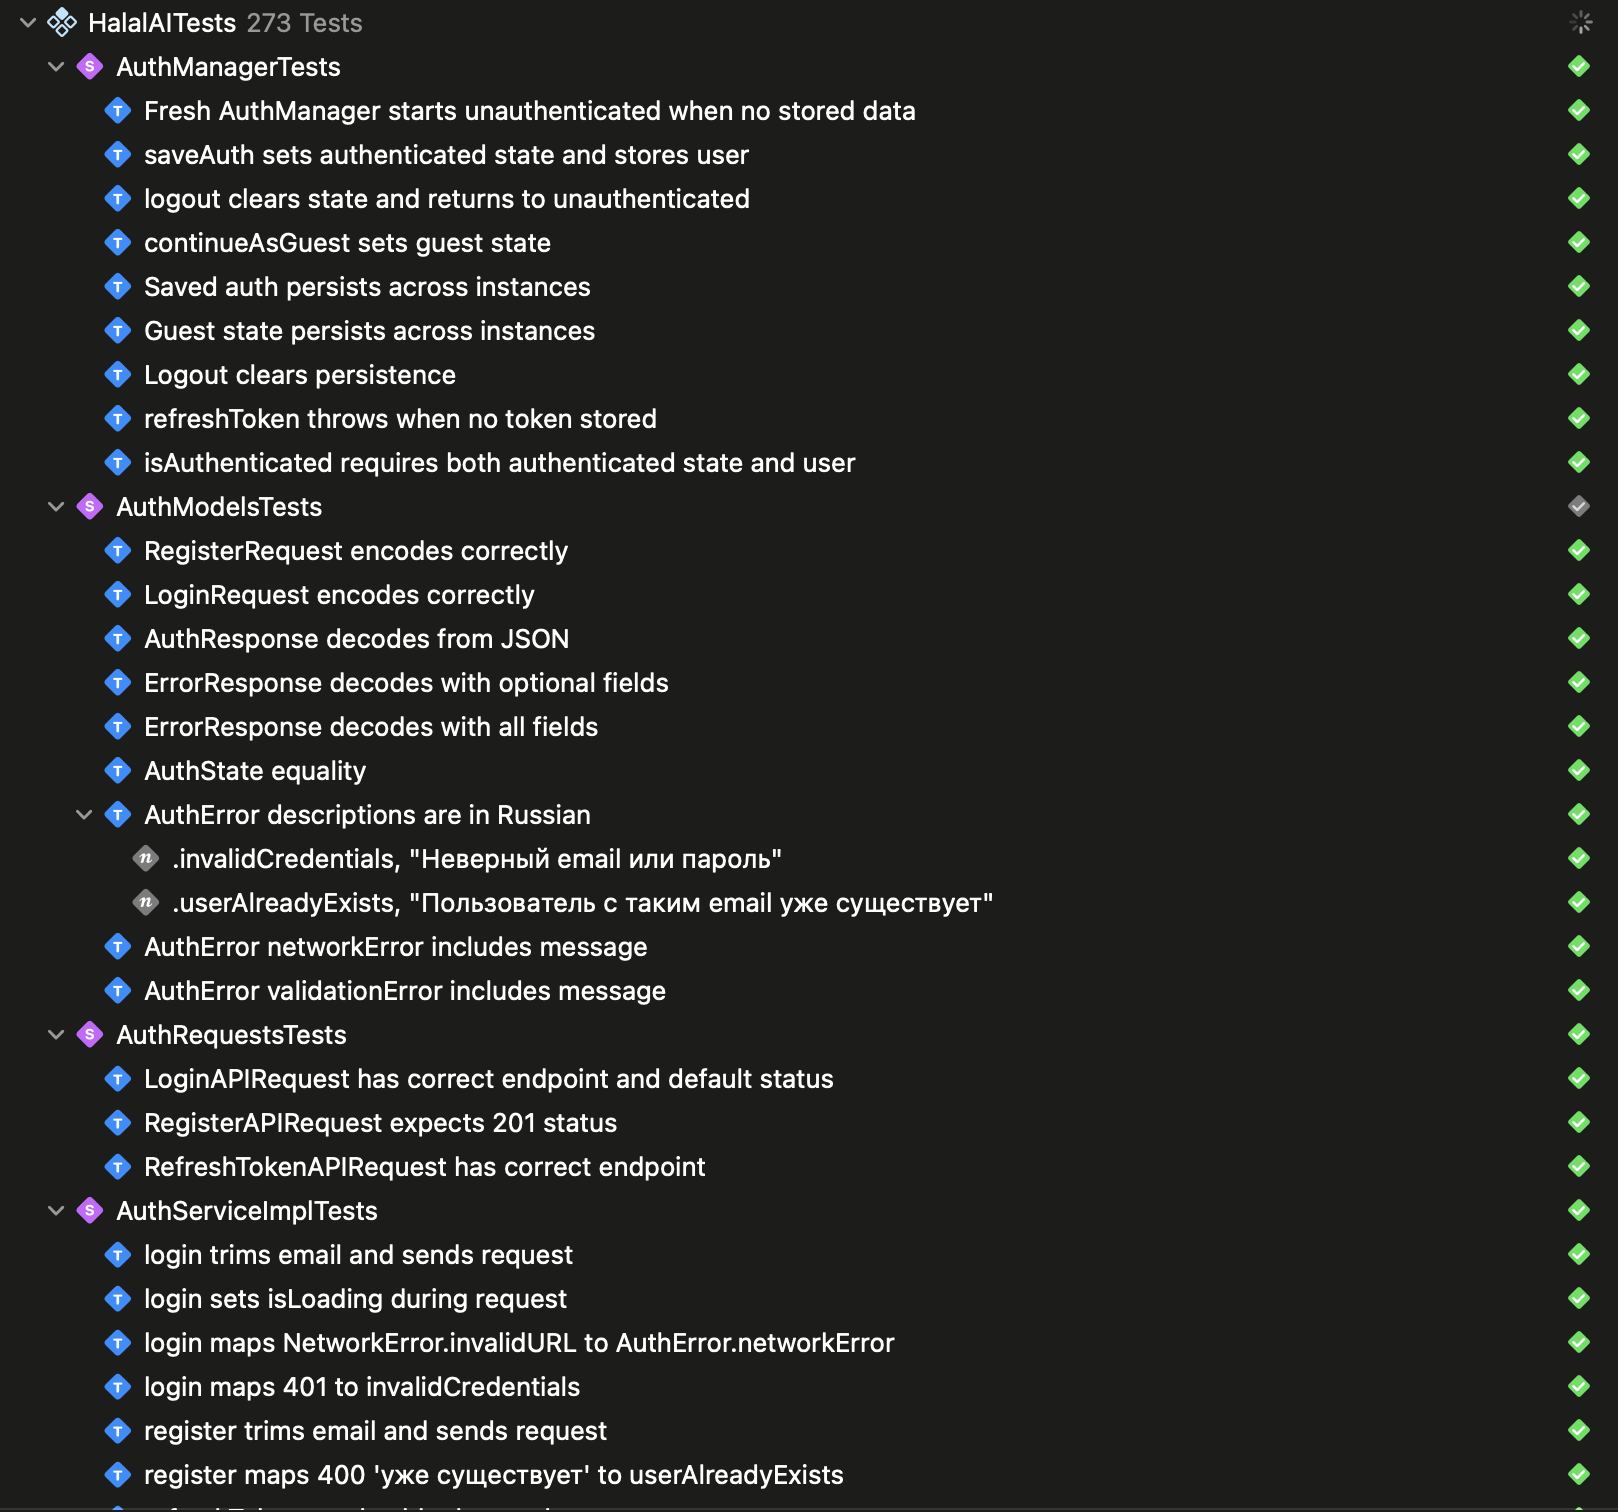
\includegraphics[width=0.85\linewidth]{my_folder/images/image41}
	\caption{iOS Unit-тесты модуля авторизации}
	\label{fig:image41}
\end{figure}


Был протестирован модуль анализа ингредиентов, так как данный компонент реализует основную функциональность приложения. Для модуля IngredientMatcher были реализованы тесты распознавания E-кодов, определения статусов <<халяль>>, <<харам>> и <<сомнительно>>, а также обработки граничных случаев пользовательского ввода. Отдельно тестировались алгоритмы оценки совпадений ингредиентов, обработка специальных символов, а также регистронезависимый поиск (рисунок~\ref{fig:42}).


\begin{figure}[H]
	\centering
	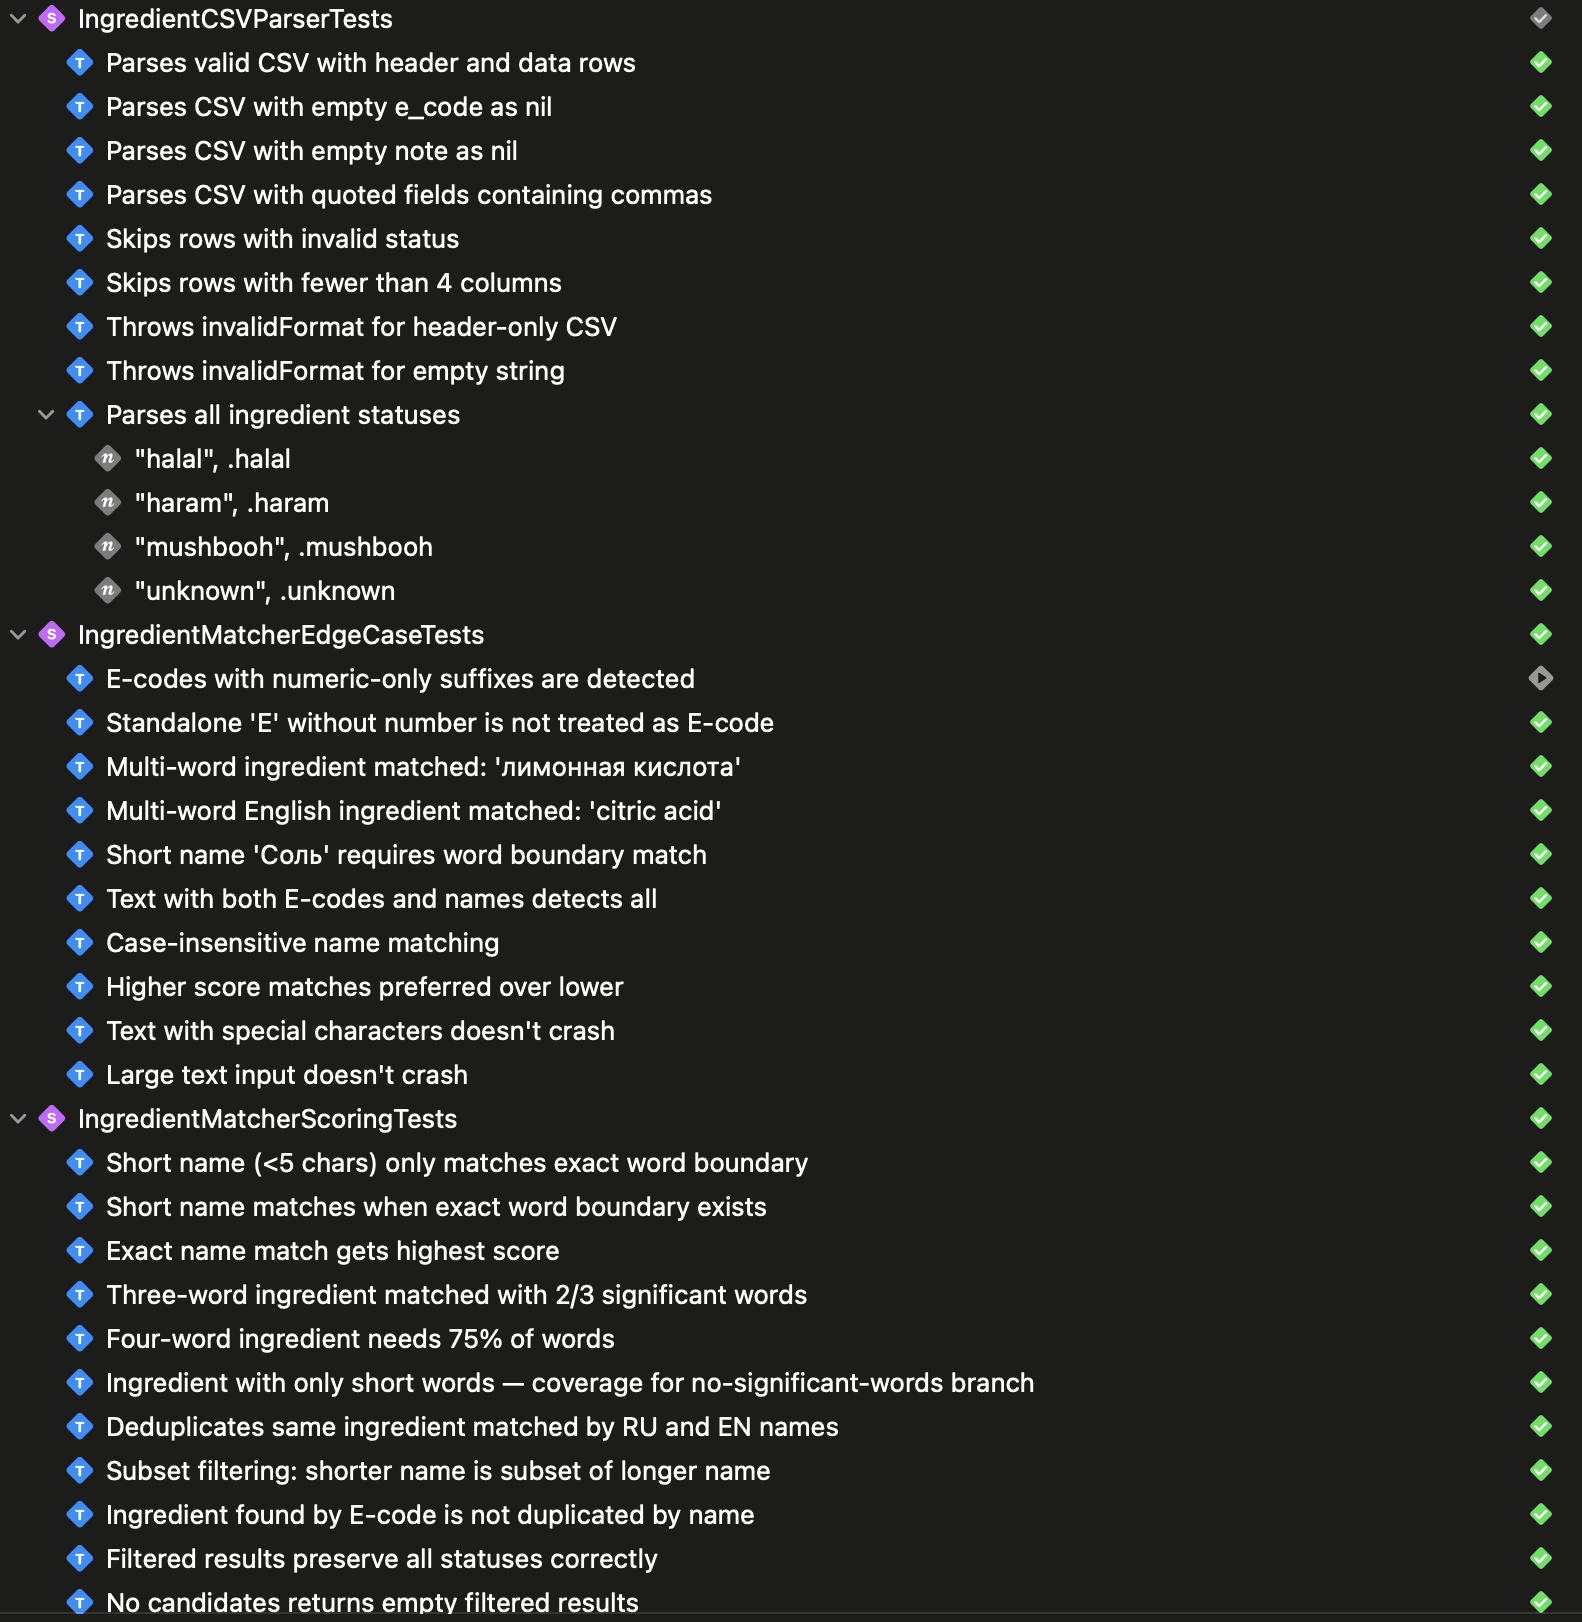
\includegraphics[width=0.85\linewidth]{my_folder/images/image42}
	\caption{iOS Unit-тесты модуля анализа ингредиентов}
	\label{fig:42}
\end{figure}


Были написаны тесты для проверки корректности расчетов времени молитв, проверялось: корректность порядка времен молитв, поддержка различных методов расчета, различия между мазхабами, корректность определения следующей молитвы (рисунок~\ref{fig:43}).


\begin{figure}[H]
	\centering
	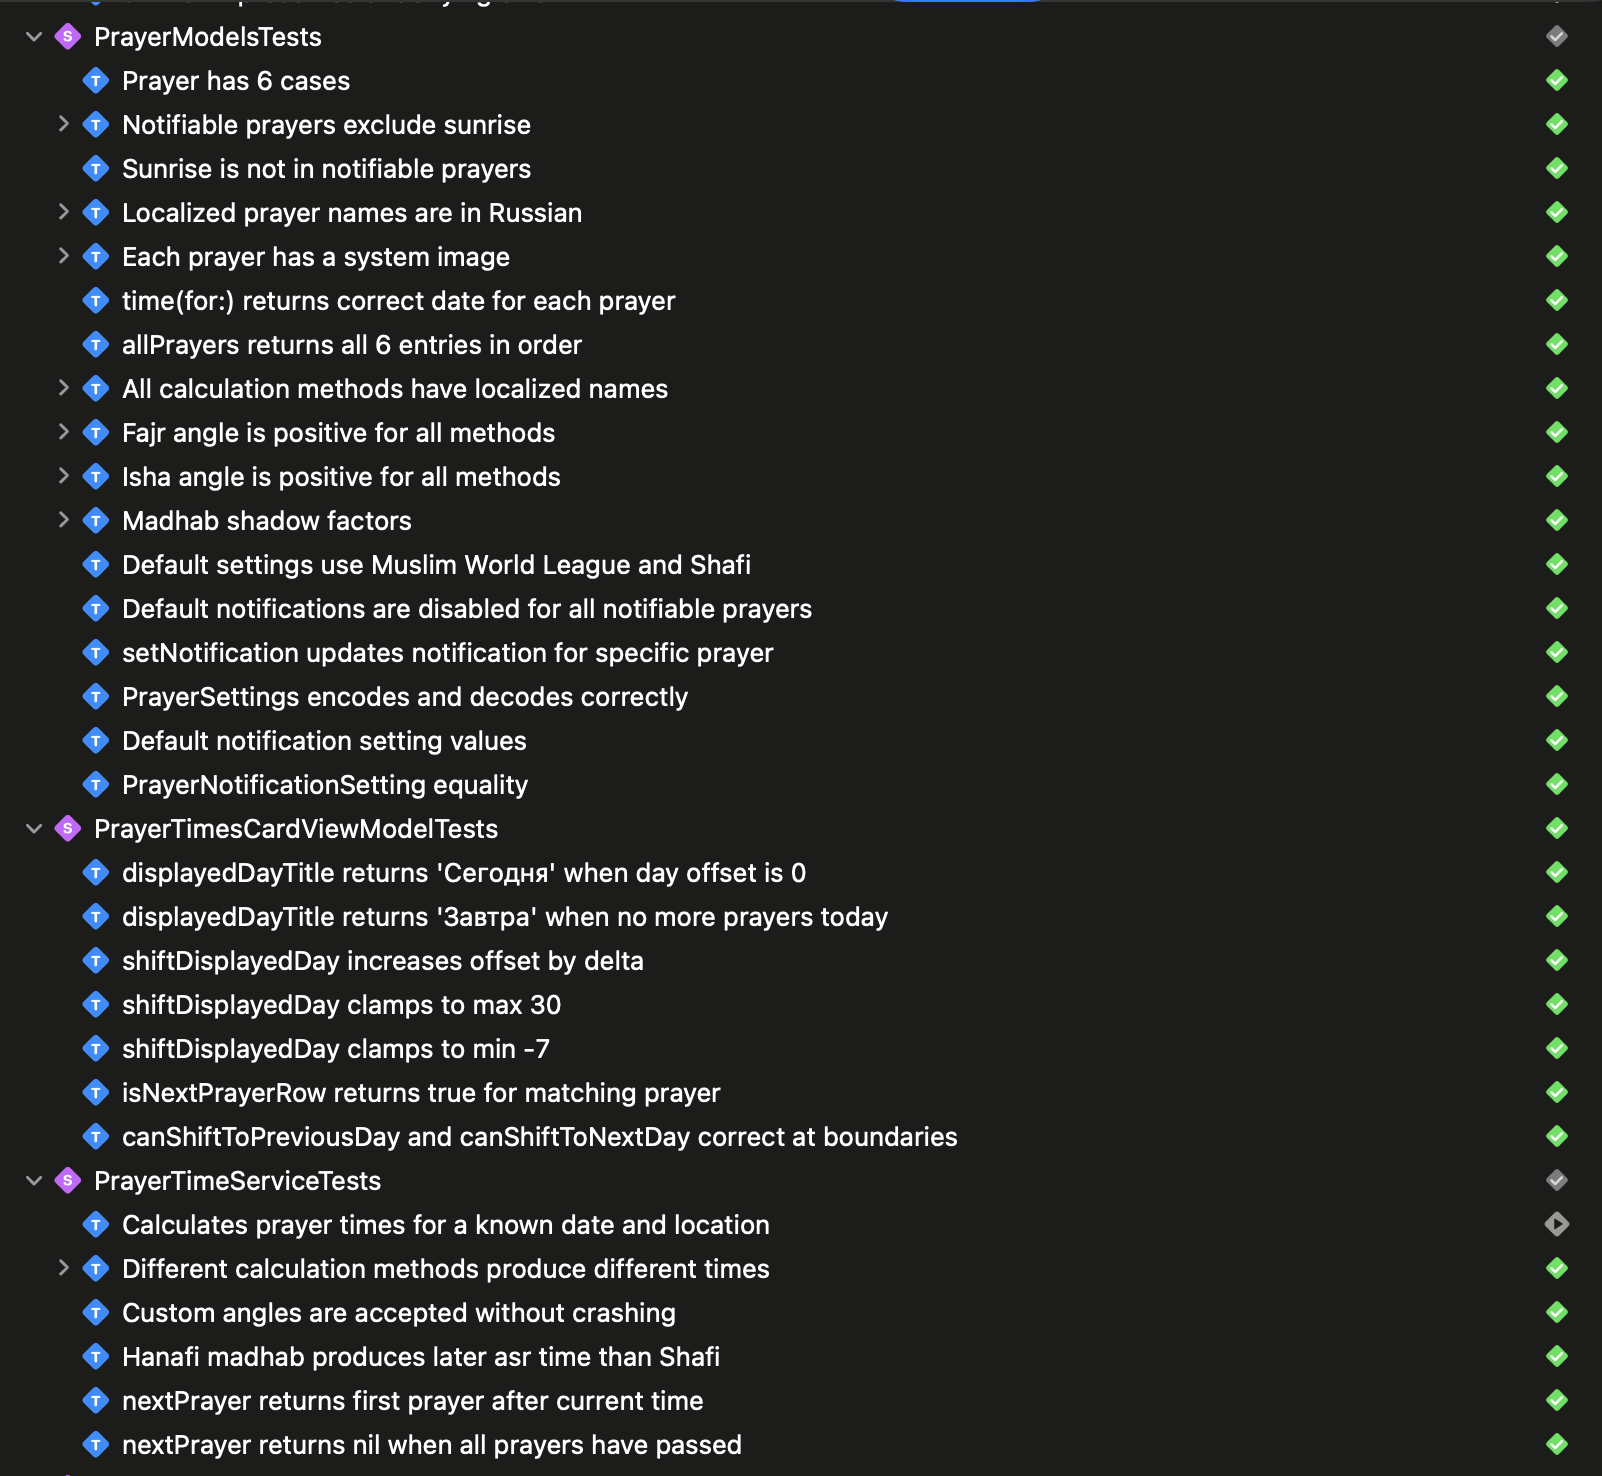
\includegraphics[width=0.85\linewidth]{my_folder/images/image43}
	\caption{iOS Unit-тесты модуля расчета времени молитв}
	\label{fig:43}
\end{figure}


Также были реализованы тесты модулей AI-чата и сетевого взаимодействия. Проверялись сценарии отправки сообщений, обработка пустого пользовательского ввода, изменение состояния соединения, загрузка доступных моделей и обработка ошибок backend-сервиса (рисунок~\ref{fig:44}).


\begin{figure}[H]
	\centering
	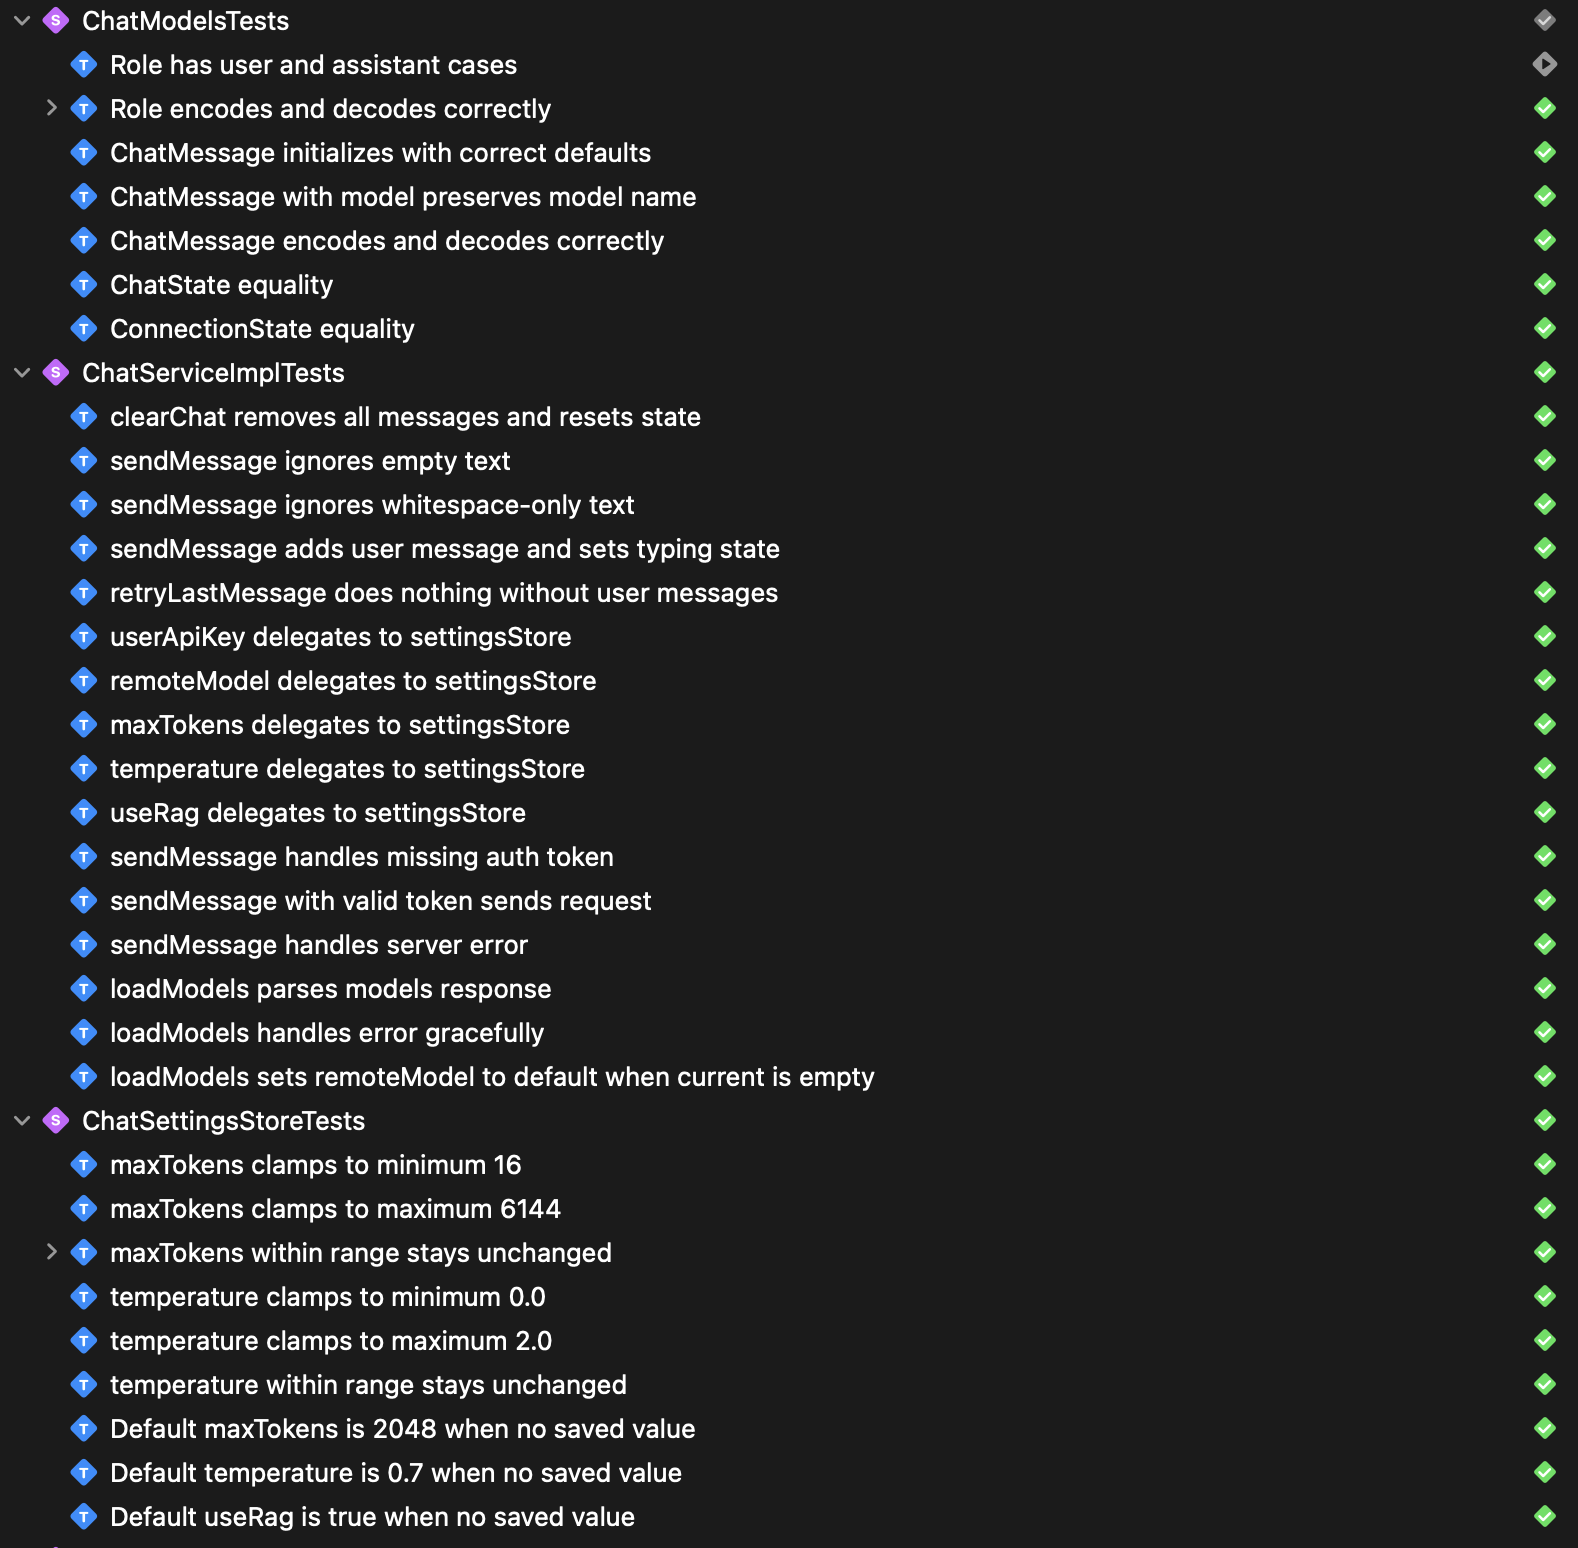
\includegraphics[width=0.85\linewidth]{my_folder/images/image44}
	\caption{iOS Unit-тесты модуля чата}
	\label{fig:44}
\end{figure}


Также было написано множество тестов для навигации приложения, механизмов кеширования пользовательских данных и ViewModel-ей более мелких экранов. Всего удалось покрыть unit-тестами 29,4\% - это 2779 из 9452 исполняемых строк. Относительно низкий процент объясняется архитектурными особенностями iOS-приложения - большая часть кода относится к слою пользовательского интерфейса, который содержит преимущественно декларативное описание интерфейса и ограниченное количество бизнес-логики, чтобы повысить процент покрытия будут написаны UI-тесты для важных экранов. Если же смотреть на покрытие бизнес-логики, то это будет 71,01\% (1369 / 1928) (рисунок~\ref{fig:45}).


\begin{figure}[H]
	\centering
	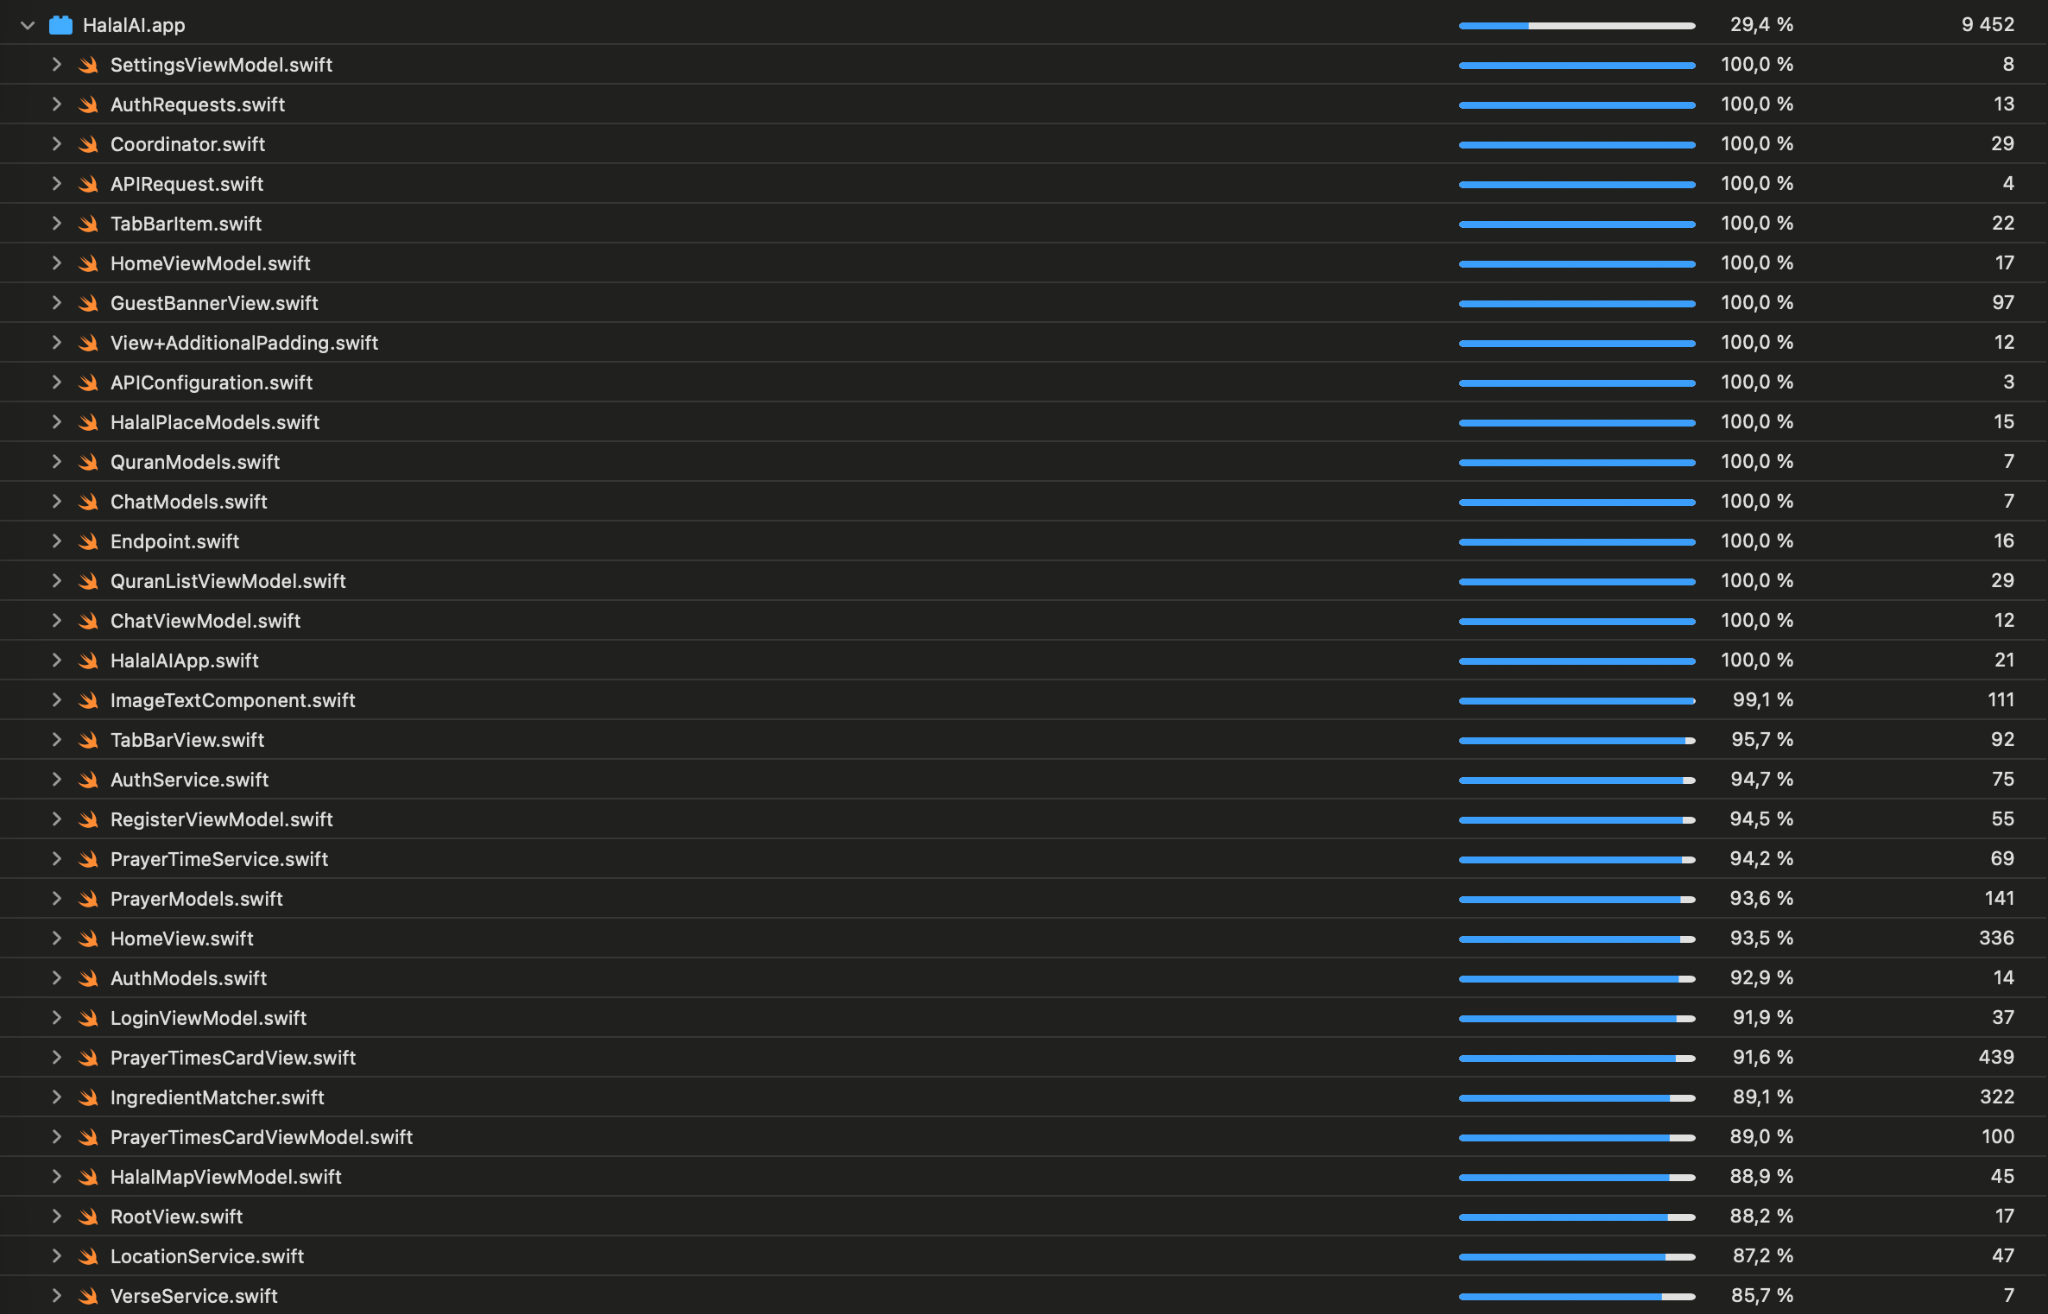
\includegraphics[width=0.85\linewidth]{my_folder/images/image45}
	\caption{iOS Unit-тесты покрытие}
	\label{fig:45}
\end{figure}


\subsection{UI-тестирование}


UI-тестирование выполнялось с помощью фреймворка XCUITest и было направлено на проверку основных пользовательских сценариев приложения. Всего было написано 28 UI-тестов, охватывающих ключевые элементы навигации и взаимодействия пользователя с системой.


Основная часть тестов была сосредоточена на проверке экранов авторизации и регистрации, навигации между табами в приложении, корректности отображения основных экранов, доступности функциональности для гостевого режима и ограничений доступа к отдельным функциям приложения (рисунок~\ref{fig:46}).


\begin{figure}[H]
	\centering
	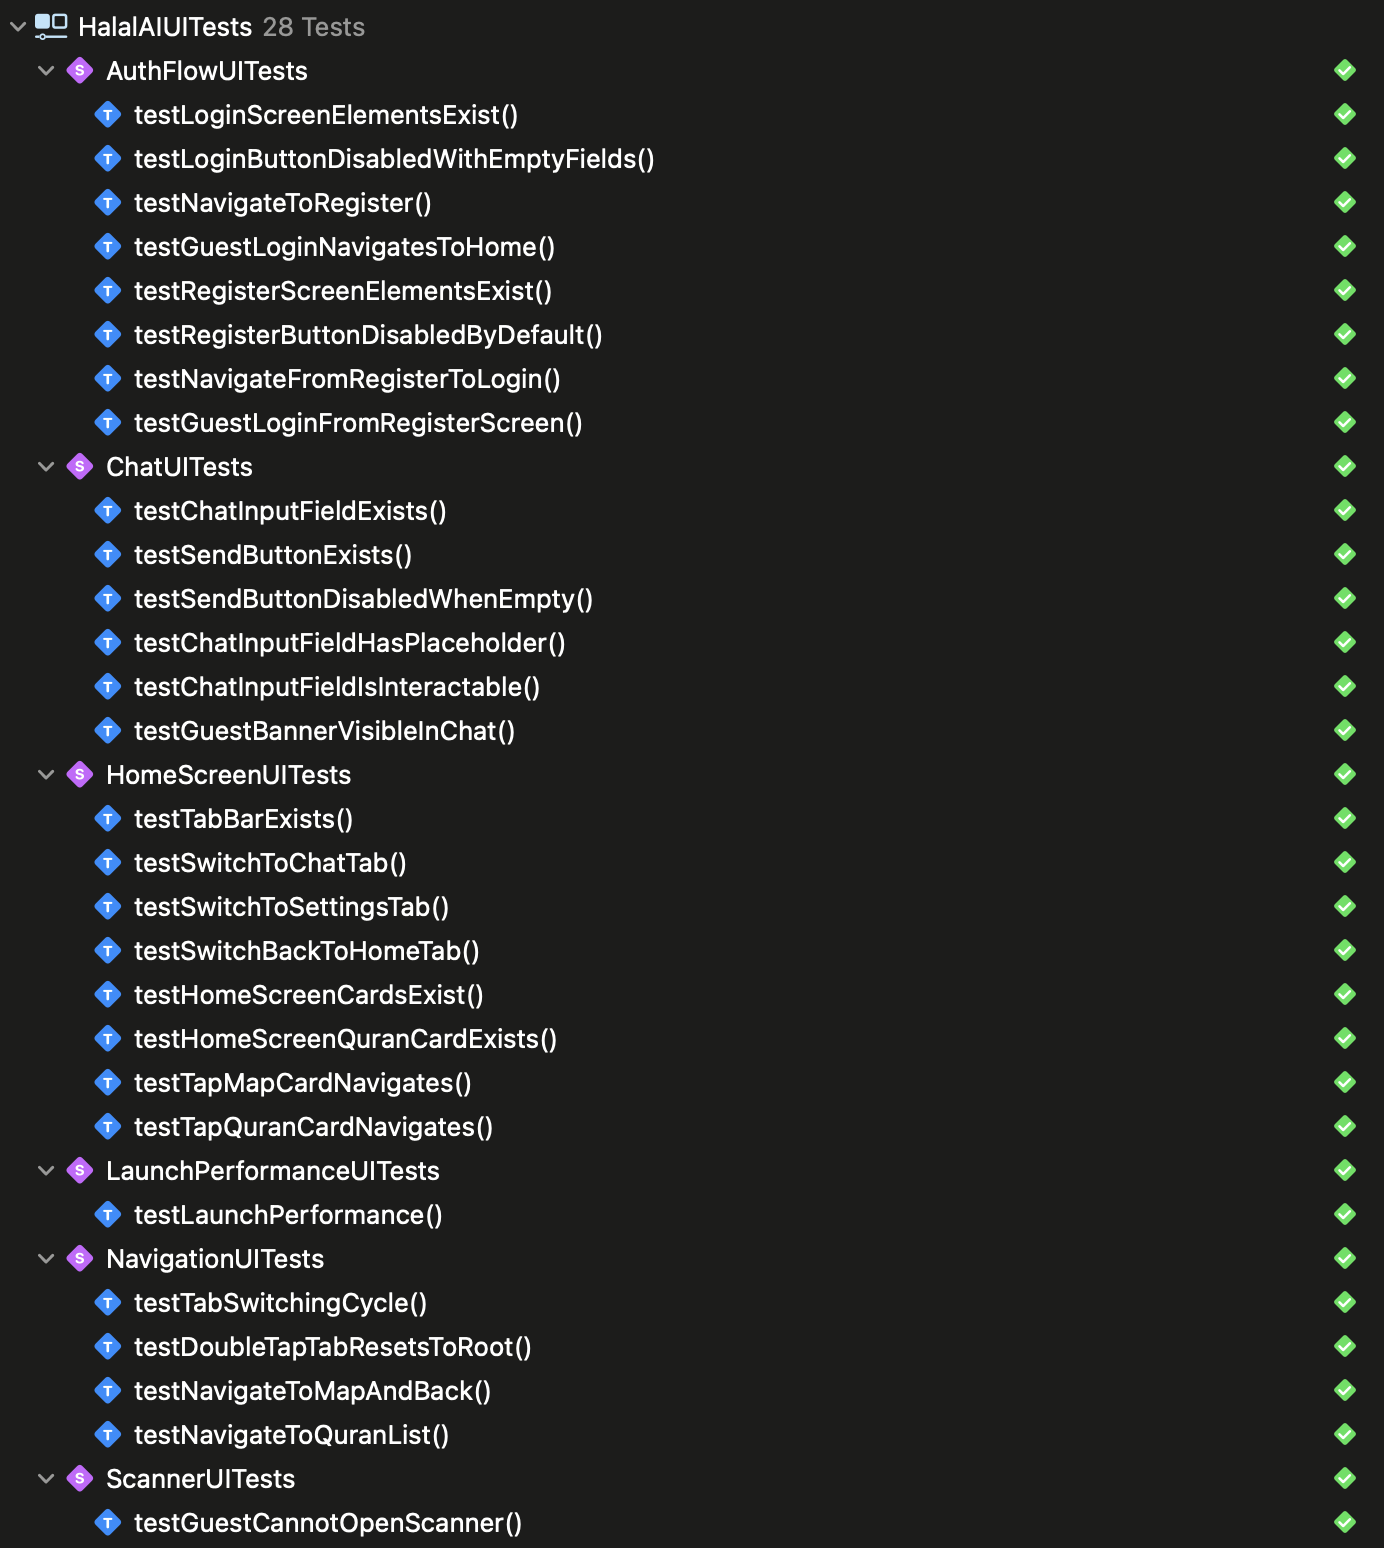
\includegraphics[width=0.85\linewidth]{my_folder/images/image46}
	\caption{iOS UI-тесты}
	\label{fig:46}
\end{figure}


После написания UI-тестов общее покрытие проекта iOS тестами увеличилось до 57.6\% (рисунок~\ref{fig:47}).


\begin{figure}[H]
	\centering
	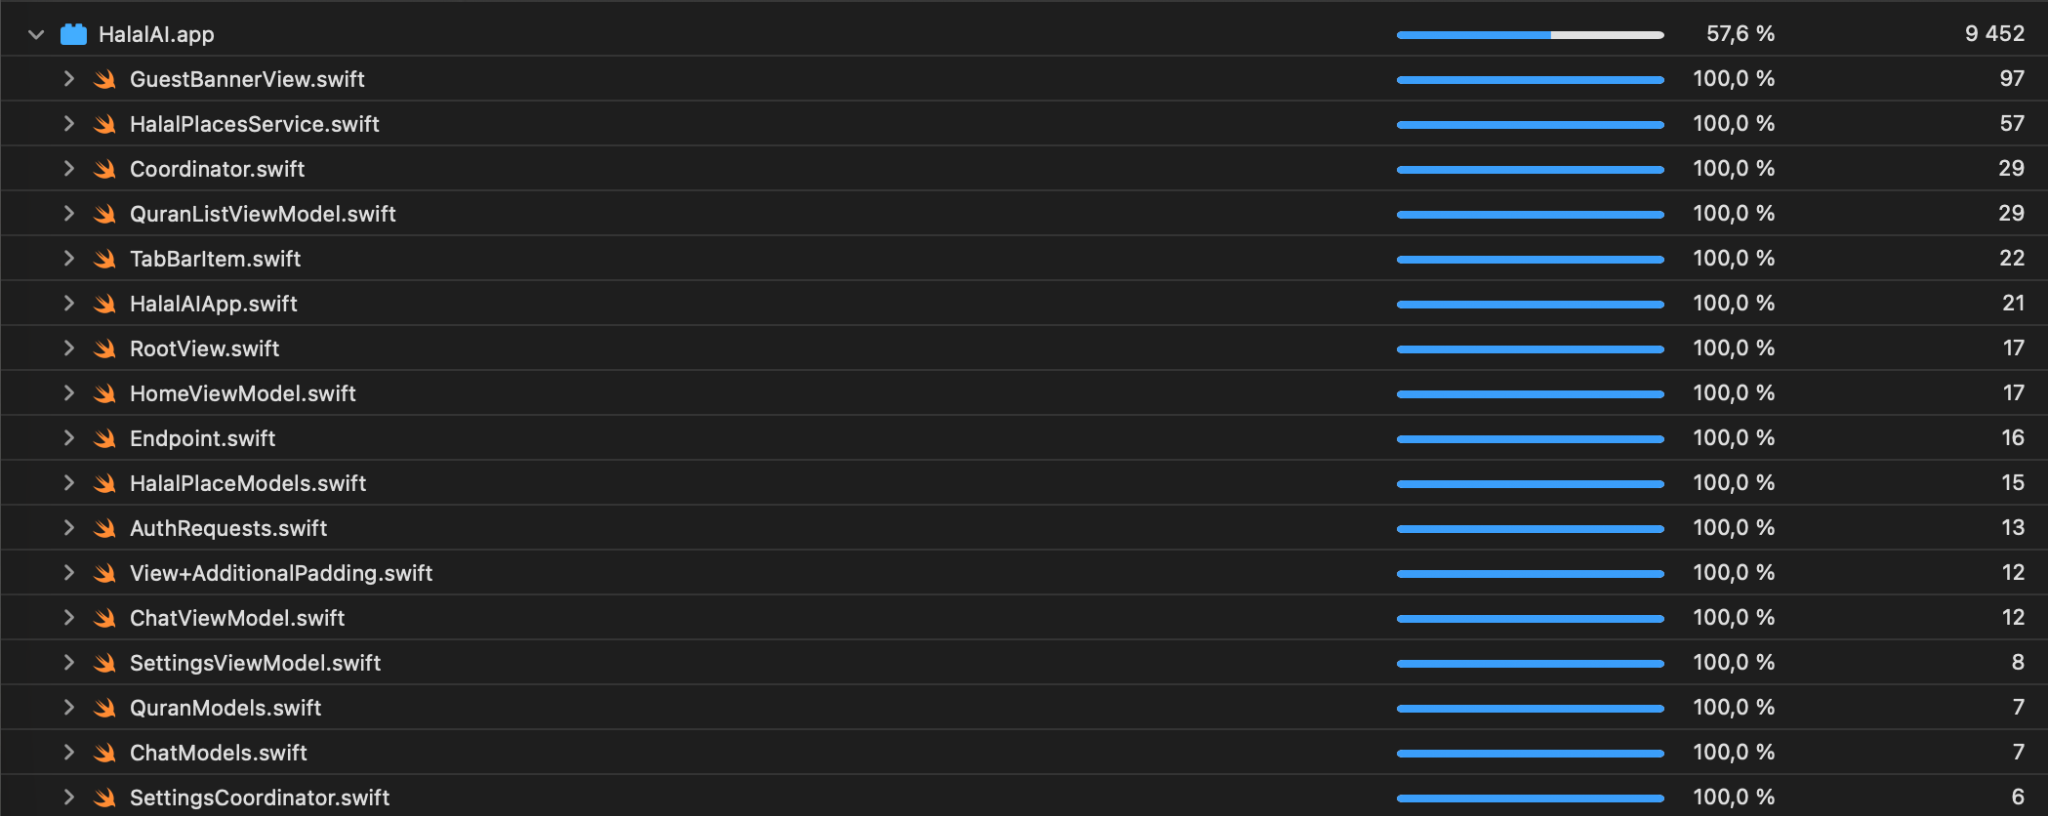
\includegraphics[width=0.85\linewidth]{my_folder/images/image47}
	\caption{Покрытие кода после написания  UI-тестов}
	\label{fig:47}
\end{figure}


\section{Тестирование backend-сервиса}


Для backend были написаны автоматизированные тесты, покрывающие основные уровни архитектуры: контроллеры, сервисы, механизмы безопасности, обработку исключений и интеграцию с внешним LLM-сервисом.


Тестирование выполнялось с использованием фреймворков Spring Boot Test, JUnit 5, Mockito и MockMvc. Для изоляции тестируемых компонентов применялись mock-объекты, это позволило проверять бизнес-логику независимо от реальных внешних зависимостей, базы данных и сетевых запросов.


Были реализованы следующие категории тестов: unit-тесты сервисного слоя, тесты REST-контроллеров, тесты JWT-аутентификации и компонентов безопасности, тесты глобального обработчика исключений, интеграционные smoke-тесты Spring Boot-приложения, тесты загрузки и обработки CSV-данных, тесты интеграции с LLM-сервисом.


Также были написаны тесты для сервиса генерации ответов от LLM-Service. Были написаны тесты успешной генерации ответа, обработки параметров генерации и различных ошибочных сценариев.


Для подсистемы аутентификации были протестированы сценарии регистрации, входа пользователя, обновления JWT-токена, обработки неверных учетных данных, блокировки отключенных пользователей и защиты от использования некорректных токенов.


Тестирование REST-контроллеров выполнялось с использованием MockMvc и включало проверку: корректности HTTP-статусов, структуры JSON-ответов, обработки ошибок валидации, корректного преобразования исключений в HTTP-ответы.


Также были написаны тесты для загрузки аятов Корана из CSV-файлов, проверки корректности парсинга данных и пропуска некорректных строк. Всего backend-часть проекта содержит 15 файлов автоматизированных тестов, покрывающих основные критические сценарии работы системы, включая безопасность, бизнес-логику и интеграцию с внешними сервисами.


Для оценки качества тестирования проекта использовался инструмент JaCoCo, позволяющий анализировать степень покрытия кода автоматизированными тестами. По результатам тестирования были получены следующие показатели покрытия (рисунок~\ref{fig:48}):

\begin{enumerate}
	\item покрытие строк кода - 100\% в анализируемом наборе классов.
	\item покрытие JVM-инструкций - 99\%.
	\item покрытие ветвлений - 88\%.
\end{enumerate}

\begin{figure}[H]
	\centering
	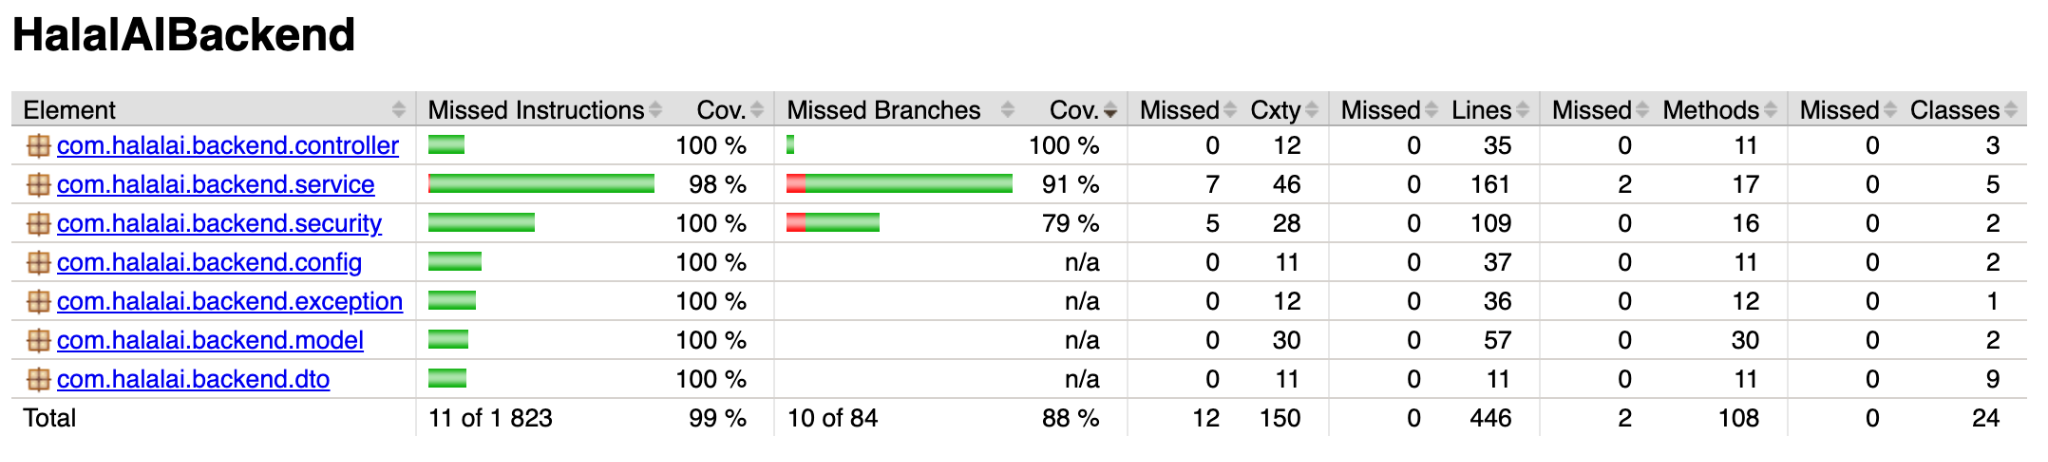
\includegraphics[width=0.85\linewidth]{my_folder/images/image48}
	\caption{Отчет JaCoCo о покрытии backend-сервиса}
	\label{fig:48}
\end{figure}


\section{Тестирование LLM-сервиса}


Тестирование LLM-сервиса проводилось с использованием фреймворка pytest. Основной целью тестирования является проверка RAG-системы, API-слоя, обработки ошибок, а также взаимодействия с внешними LLM-провайдерами. Были написаны Unit и интеграционные тесты. Unit тесты проверяли компоненты системы в изоляции от внешних зависимостей. Для этого использовались mock-объекты SentenceTransformer, SimpleRAG, OpenRouterClient и других сервисов. Интеграционные тесты проверяли работу HTTP-API FastAPI-приложения и взаимодействие компонентов между собой. Для ускорения и стабильности тестирования реальные embedding-модели и внешние LLM-запросы также заменялись mock-объектами.


Для VectorStore были написаны тесты, проверяющие работу поиска документов, корректность вычисления косинусной близости, обработку пустого хранилища, корректную работу параметра top\_k, а также добавление новых документов и объединение embedding-векторов.


Для SimpleRAG тестировался поиск релевантных документов, обработка пустых запросов, ранжирование найденных результатов и корректное взаимодействие с embedding-моделью.


В сервисе обработки чатов ChatService были протестированы: извлечение пользовательского сообщения из истории диалога, формирование prompt, обработка отсутствующих сообщений, работа RAG, обработка ошибок OpenRouter API, обработка пустого ответа модели, сценарии работы без API-ключа, отключение и включение RAG-поиска.


Для OpenRouterClient были реализованы тесты успешного взаимодействия с API, обработки HTTP-ошибок, проверки корректности JSON-структуры ответа, формирования HTTP-заголовков и корректного использования системного prompt.


Для интеграционного тестирования API использовался FastAPI TestClient, это позволило не запускать отдельно сервер. Проверялись HTTP-коды ответа (200, 400, 422, 503), структура JSON-ответов и корректность обработки ошибок (рисунок~\ref{fig:49}).


\begin{figure}[H]
	\centering
	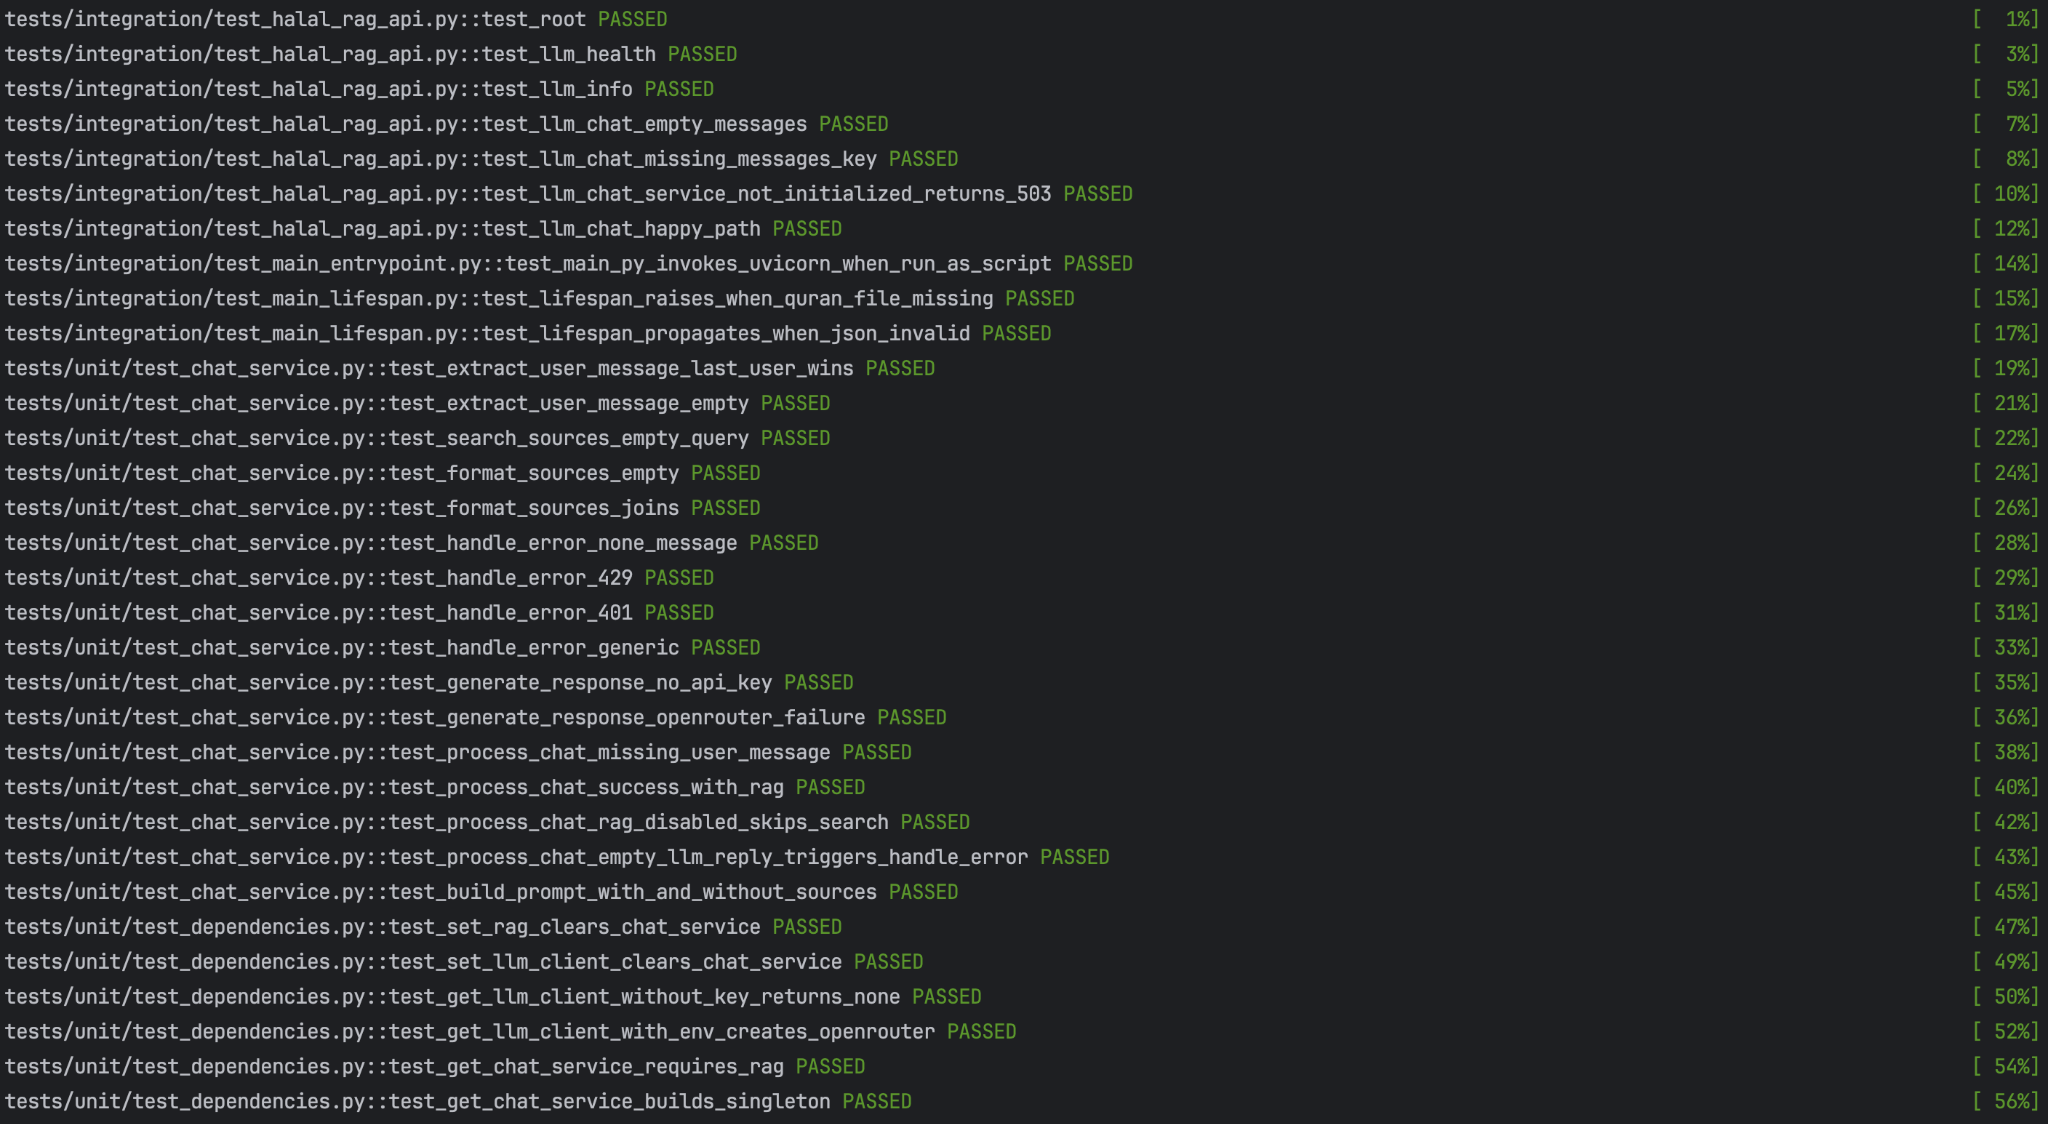
\includegraphics[width=0.85\linewidth]{my_folder/images/image49}
	\caption{Отчет JaCoCo о покрытии backend-сервис}
	\label{fig:49}
\end{figure}


По результатам выполнения тестов было достигнуто 100\% покрытие строк кода для основных модулей LLM-сервиса. Всего было покрыто 381 исполняемое выражение. Часть интерфейсных классов была исключена из расчета покрытия, поскольку они содержат только абстрактные объявления и не включают исполняемую бизнес-логику (рисунок~\ref{fig:50}).


\begin{figure}[H]
	\centering
	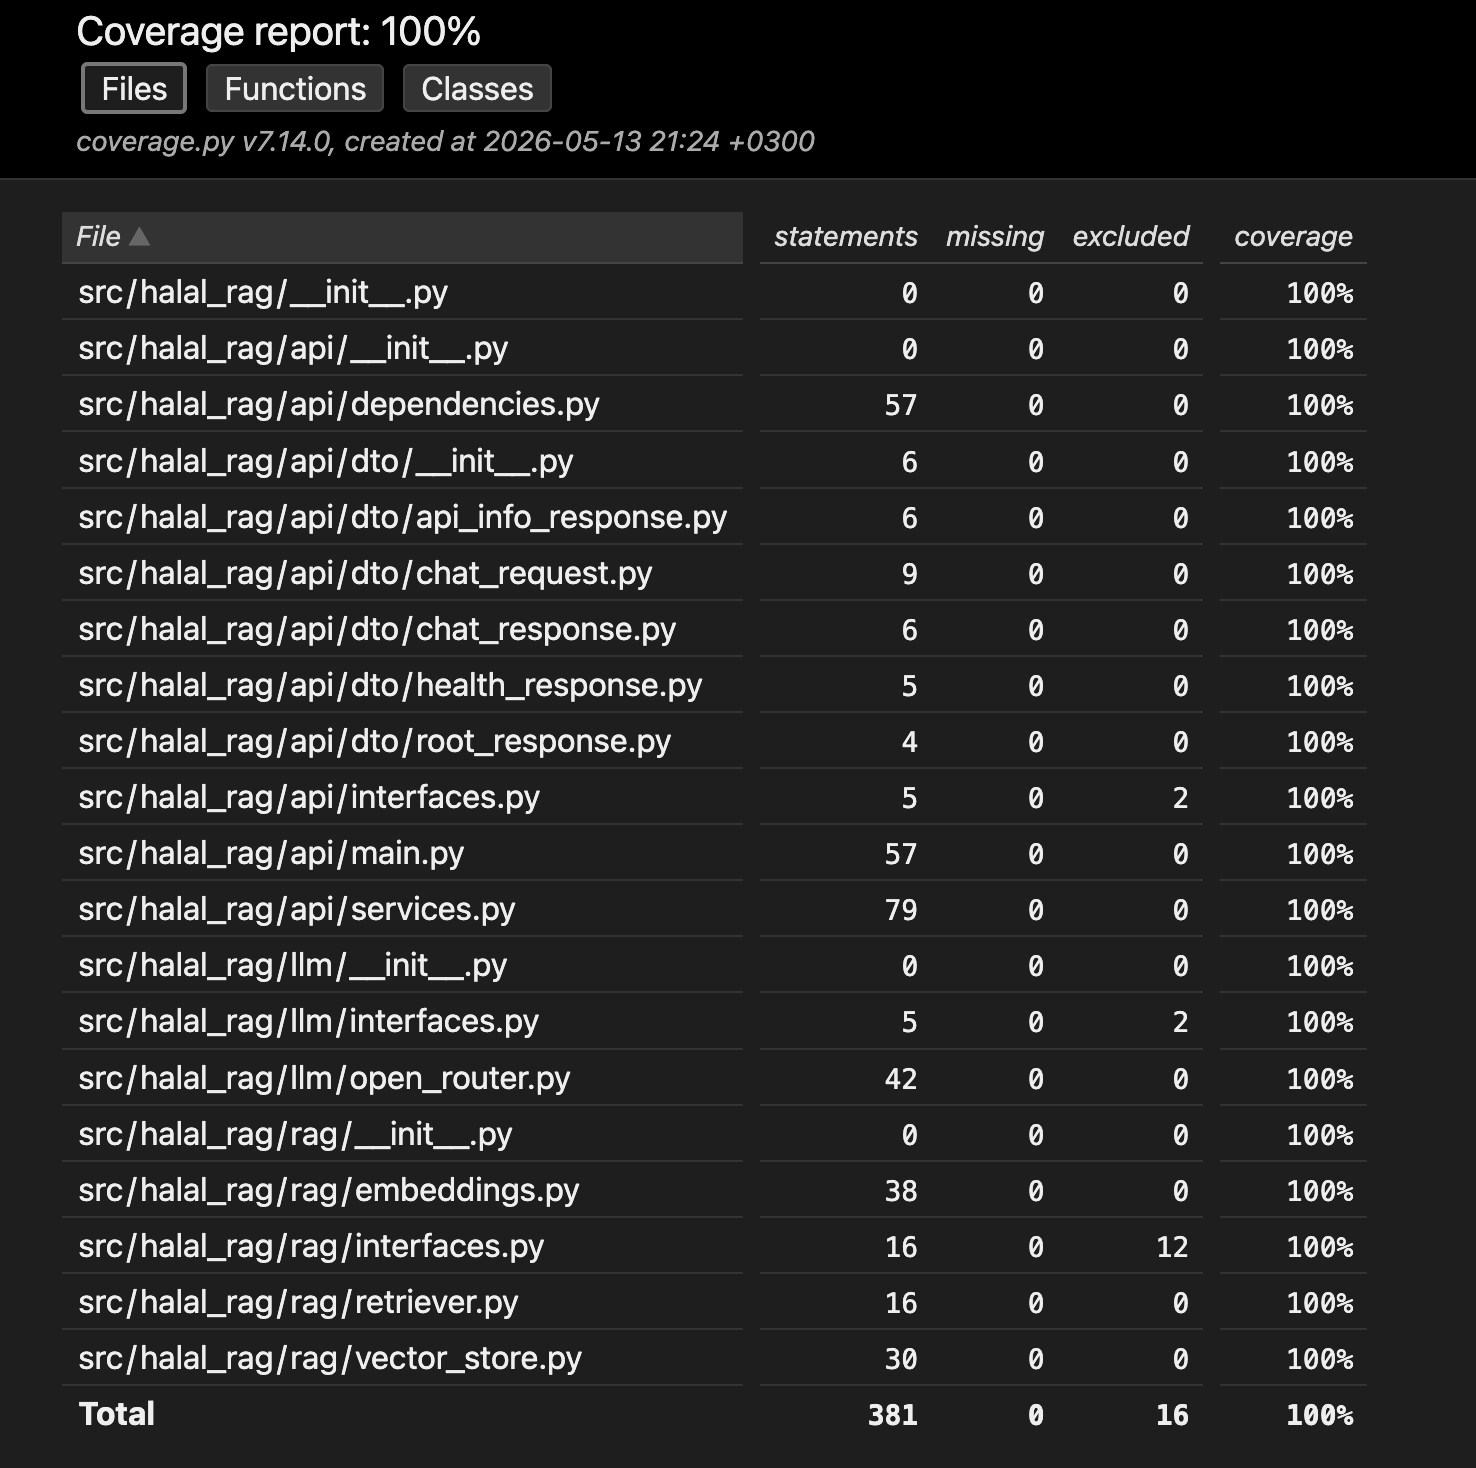
\includegraphics[width=0.85\linewidth]{my_folder/images/image50}
	\caption{Отчет pytest о покрытии LLM-service}
	\label{fig:50}
\end{figure}


Также, хочется отметить что проверка качества системы осуществлялась не только посредством классического тестирования программного обеспечения, но и в рамках экспериментального исследования, проведенного на этапе разработки LLM-сервиса. В разделе 3.2.2 выполнялась проверка сформулированных гипотез, связанных с влиянием RAG-подсистемы, embedding-моделей и их дообучения на качество генерации ответов. Для этого были проведены эксперименты с различными конфигурациями системы и выполнена оценка качества retrieval-подсистемы и итоговых ответов языковой модели по набору критериев.


\section{Проверка соответствия требованиям}


\subsection{Проверка качества распознавания состава продукта}


Для проверки использовалось ручное тестирование. Для этого использовались продуктовые упаковки и было проведено сканирование состава через приложение. Результаты приведены в таблице~\ref{tab:ocr-results}.


\begin{longtable}{|>{\small}p{1cm}|>{\small}p{2cm}|>{\small}p{5cm}|>{\small}p{4cm}|>{\small}p{2cm}|}
	\caption{Результаты распознавания состава продуктов}\label{tab:ocr-results}\\
	\hline
		No. & Продукт & Состав на упаковке & Распознано системой & \% совпадения \\
	\hline
	\endfirsthead
	\captionsetup{format=tablenocaption,labelformat=continued}
	\caption[]{}\\
	\hline
		No. & Продукт & Состав на упаковке & Распознано системой & \% совпадения \\
	\hline
	\endhead
	\hline
	\endfoot
	\hline
	\endlastfoot
		1 & Мармелад & Патока, сахар, вода, желатин, регулятор кислотности (лимонная кислота), концентрированный яблочный сок, масло пальмовое, сироп карамельный, ароматизаторы натуральные, глазирователь, красители (антоцианы, экстракт паприки, куркумин). & сахар, патока, желатин, антоцианы, ароматизаторы, лимонная кислота, пальмовое масло, вода. & 72\% \\
	\hline
		2 & Бекон & Грудореберная часть свинная, ширицовочный рассол (вода питьевая, комплексная пищевая добавка для мясной продукции с йодом (соль пищевая); фиксатор окраски нитрит натрия; йодат калия; агент антислеживающий Е5З8), соль пищевая выварочная йодированная (соль пищевая выварочная, йодат калия, агент антислеживающий Е5З8), комплексная пищевая добавка (регулятор кислотности Е4351, стабилизатор Е4501), комплексная пищевая добавка (консервант Е2622(1)), регуляторы кислотности (Е327, Е331(1)(II)), пищевая добавка (загуститель Е407А), белок говяжий животный, комплексная пищевая добавка (ароматизатор <<говядина>> (вещества вкусоароматические), усилитель вкуса и аромата Е621, сухая патока глюкозы, декстроза, соль, лактоза), жидкий ароматизатор (масло чеснока, натуральный ароматизатор чеснока), пищевая добавка (агент желирующий Е850), пищевая добавка (антислеживающий Е300), пищевая добавка (загуститель Е415). & глютен, патока, лактоза, (часть) свинная, декстроза, нитрит натрия, нитрит калия, вода, соль & 38\% \\
	\hline
		3 & Хлеб & вода, натуральная мука ржаная хлебопекарная обдирная, мука пшеничная хлебопекарная первого сорта, соль, дрожжи хлебопекарные & пшеничная мука, вода, мука, соль & 100\% \\
\end{longtable}


В ходе тестирования была проведена проверка работы системы распознавания состава продуктов на основе реальных упаковок и их сканирования через приложение (рисунок~\ref{fig:51}).


Полученные значения показывают, что система в целом корректно определяет ключевые ингредиенты продуктов, однако уровень совпадения варьируется в зависимости от сложности состава. Наилучший результат был достигнут для простого состава (хлеб), где совпадение составило 100\%, что свидетельствует о высокой точности распознавания базовых ингредиентов. Для более сложных продуктов (мармелад и бекон) наблюдается снижение процента совпадения. Это связано с наличием комплексных пищевых добавок, вложенных составов и технологических компонентов (E-добавок), не всегда явно интерпретируемых системой. Следует отметить, что система распознавания ориентирована не на полное восстановление состава продукта, а на выделение ключевых ингредиентов с точки зрения классификации по категориям халяль, харам и сомнительных компонентов.


\begin{figure}[H]
	\centering
	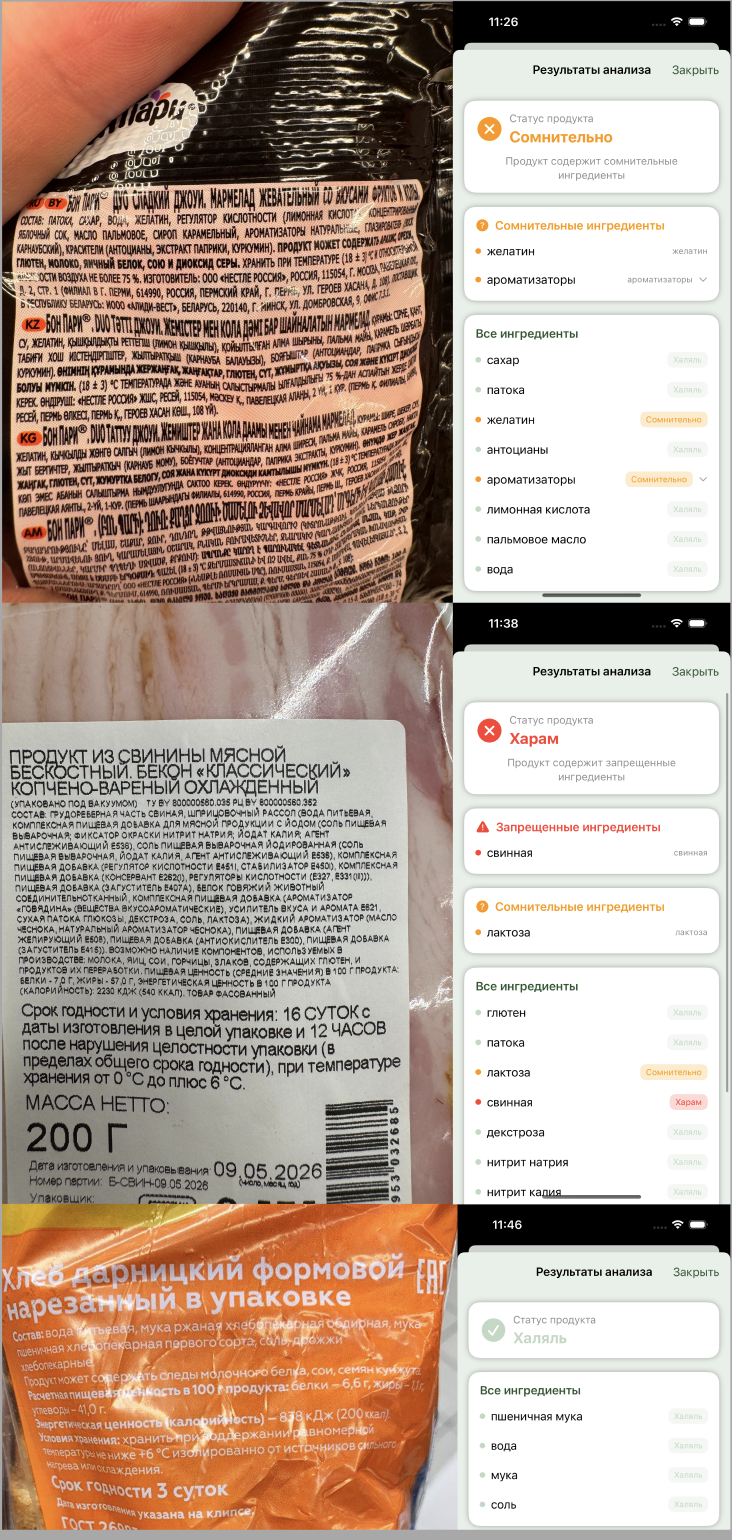
\includegraphics[width=0.85\linewidth, height=0.85\textheight, keepaspectratio]{my_folder/images/image51}
	\caption{Сканирование реальных составов через приложение}
	\label{fig:51}
\end{figure}


\subsection{Проверка корректности классификации ингредиентов}


Для проверки корректности классификации ингредиентов были написаны Unit тесты. Объектом тестирования служил компонент IngredientMatcher. Результаты представлены в таблице~\ref{tab:classification}.


\begin{longtable}{|>{\small}p{0.7cm}|>{\small}p{3.1cm}|>{\small}p{2.1cm}|>{\small}p{2.9cm}|>{\small}p{3.1cm}|>{\small}p{1.8cm}|}
	\caption{Результаты классификации ингредиентов}\label{tab:classification}\\
	\hline
		No. & Наименование теста & Входные данные & Ожидаемый результат & Фактический результат & Статус \\
	\hline
	\endfirsthead
	\captionsetup{format=tablenocaption,labelformat=continued}
	\caption[]{}\\
	\hline
		No. & Наименование теста & Входные данные & Ожидаемый результат & Фактический результат & Статус \\
	\hline
	\endhead
	\hline
	\endfoot
	\hline
	\endlastfoot
		1 & Классификация халяль-ингредиента по E-коду & E100 & Статус: Халяль & Статус: Халяль & Пройден \\
	\hline
		2 & Классификация харам-ингредиента по E-коду & E120 & Статус: Харам & Статус: Харам & Пройден \\
	\hline
		3 & Классификация мушбух-ингредиента по E-коду & E471 & Статус: Мушбух & Статус: Мушбух & Пройден \\
	\hline
		4 & Классификация харам-ингредиента по названию на русском & желатин свиной & Статус: Харам & Статус: Харам & Пройден \\
	\hline
		5 & Классификация харам-ингредиента по названию на английском & pork gelatin & Статус: Харам & Статус: Харам & Пройден \\
	\hline
		6 & Классификация мушбух-ингредиента по названию & на\-ту\-раль\-ный аро\-ма\-ти\-за\-тор & Статус: Мушбух & Статус: Мушбух & Пройден \\
	\hline
		7 & Приоритет харам над халяль & E100, E120 & Итоговый статус: Харам & Итоговый статус: Харам & Пройден \\
	\hline
		8 & Приоритет харам над мушбух & E120, E471 & Итоговый статус: Харам & Итоговый статус: Харам & Пройден \\
	\hline
		9 & Приоритет мушбух над халяль при отсутствии харам & E100, E471 & Итоговый статус: Мушбух & Итоговый статус: Мушбух & Пройден \\
	\hline
		10 & Полная цепочка приоритетов: харам > мушбух > халяль & E100, E471, E120 & Итоговый статус: Харам, обнаружено 3 ингредиента & Итоговый статус: Харам, обнаружено 3 ингредиента & Пройден \\
	\hline
		11 & Ингредиент, отсутствующий в базе данных & E999 & Статус: Неизвестно, список пуст & Статус: Неизвестно, список пуст & Пройден \\
\end{longtable}


Система корректно классифицирует ингредиенты по всем статусам как по E-коду, так и по текстовому названию. Соблюдается иерархия приоритетов - харам > мушбух > халяль > неизвестно. Все тесты пройдены успешно (рисунок~\ref{fig:52}).

\begin{figure}[H]
	\centering
	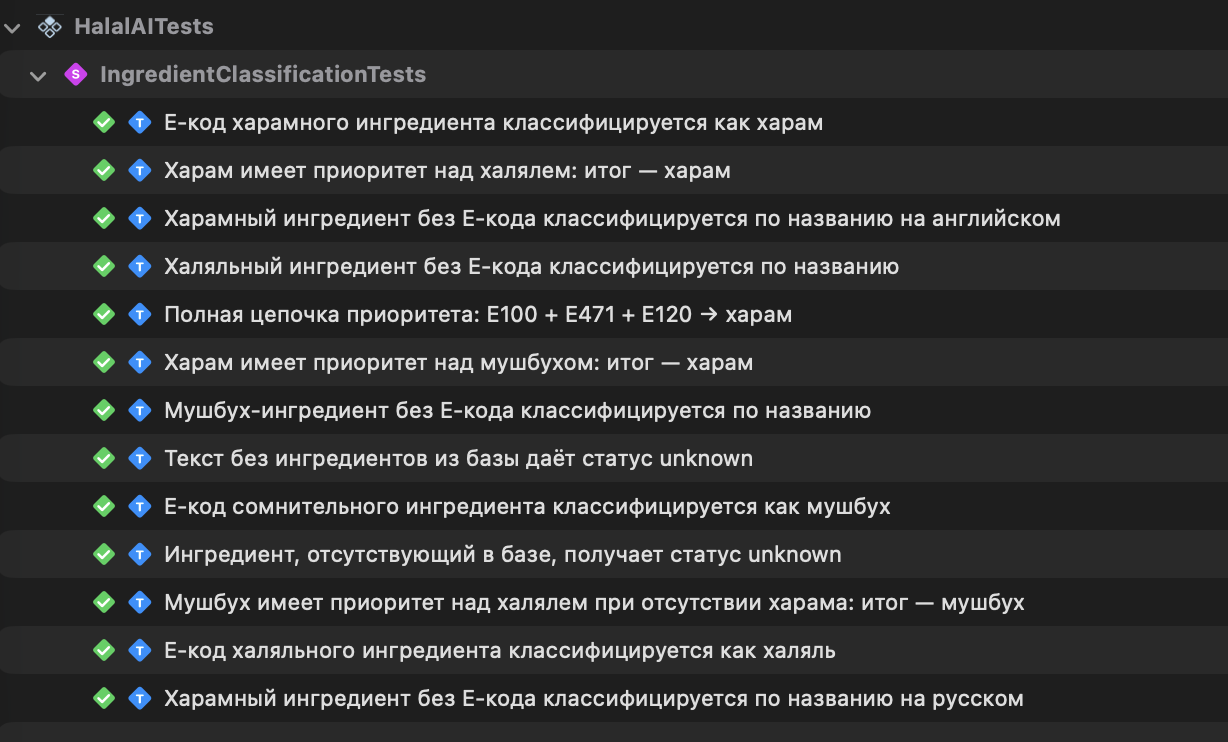
\includegraphics[width=0.85\linewidth]{my_folder/images/image52}
	\caption{Результаты прохождения тестов для IngredientMatcher}
	\label{fig:52}
\end{figure}


\subsection{Проверка реализации других модулей приложения}


В приложении успешно реализован чат с AI-ассистентом, отвечающим на вопросы пользователей на основе текстов Корана (рисунок~\ref{fig:53}). В приложении также реализован модуль чтения Корана, обеспечивающий доступ ко всем сурам и аятам, настройку размера текста и возможность продолжения чтения с последнего сохраненного места (рисунок~\ref{fig:54}). Также была реализована гибкая система настройки уведомлений о времени намаза с учетом выбранного пользователем мазхаба и метода расчета времени молитв (рисунок~\ref{fig:55}). Дополнительно в приложение была внедрена система локализации, обеспечивающая поддержку нескольких языков интерфейса и адаптацию контента в соответствии с языковыми предпочтениями пользователя (рисунки~\ref{fig:56},~\ref{fig:57}).


\begin{figure}[H]
	\centering
	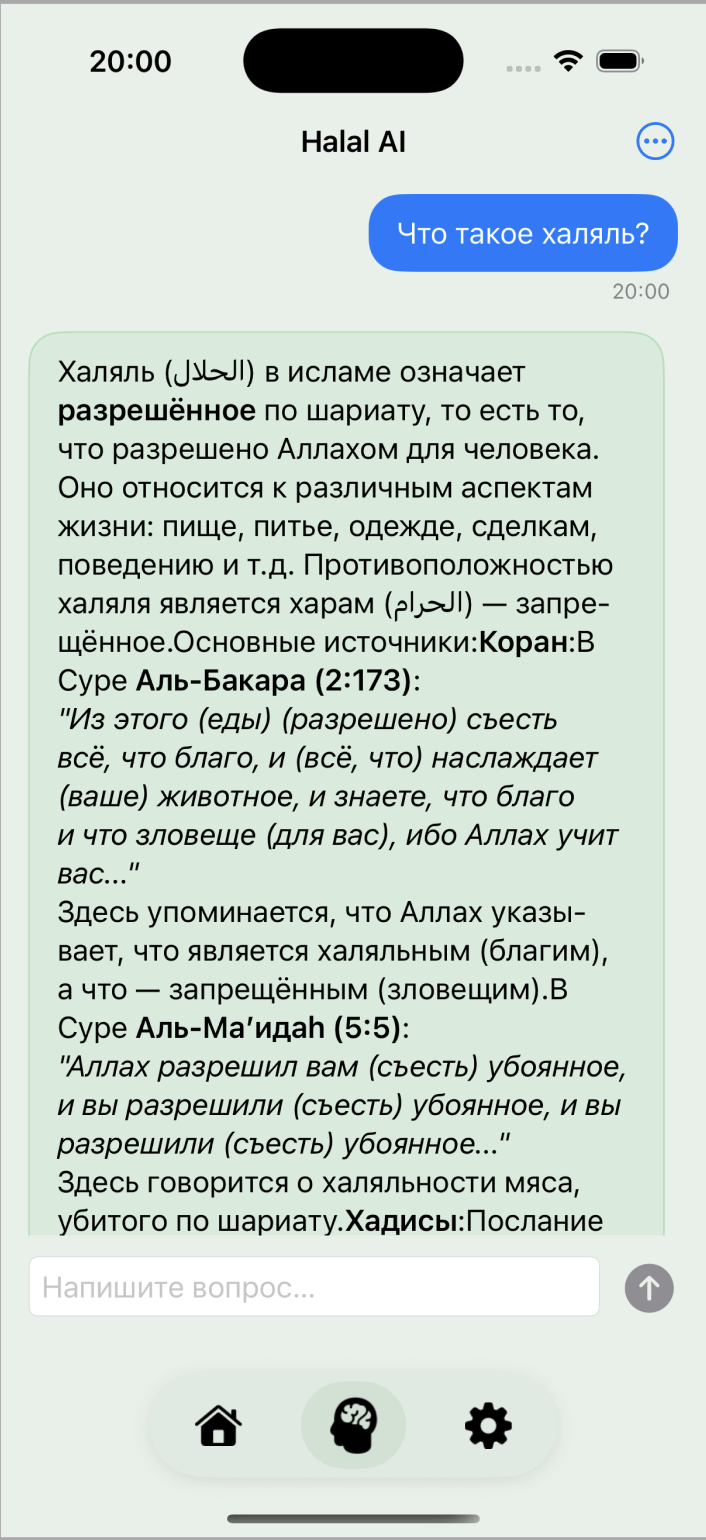
\includegraphics[width=0.85\linewidth, height=0.85\textheight, keepaspectratio]{my_folder/images/image53}
	\caption{Реализованный экран с AI-ассистентом}
	\label{fig:53}
\end{figure}


\begin{figure}[H]
	\centering
	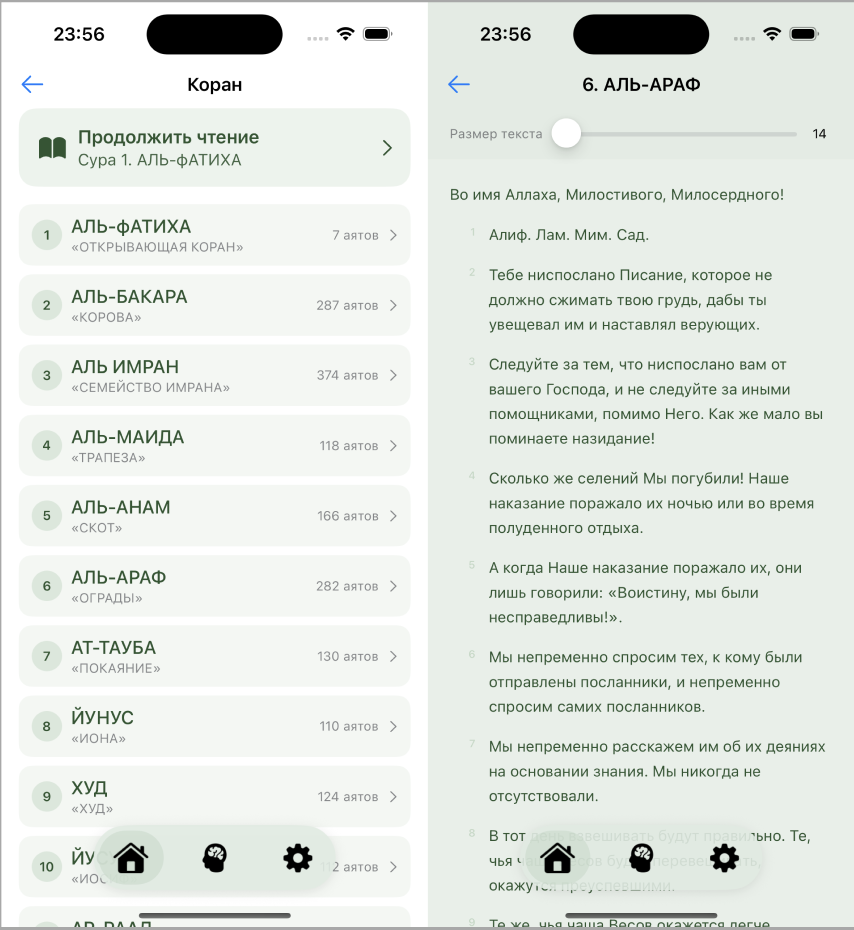
\includegraphics[width=0.85\linewidth]{my_folder/images/image54}
	\caption{Реализованный экран чтения Корана}
	\label{fig:54}
\end{figure}


\begin{figure}[H]
	\centering
	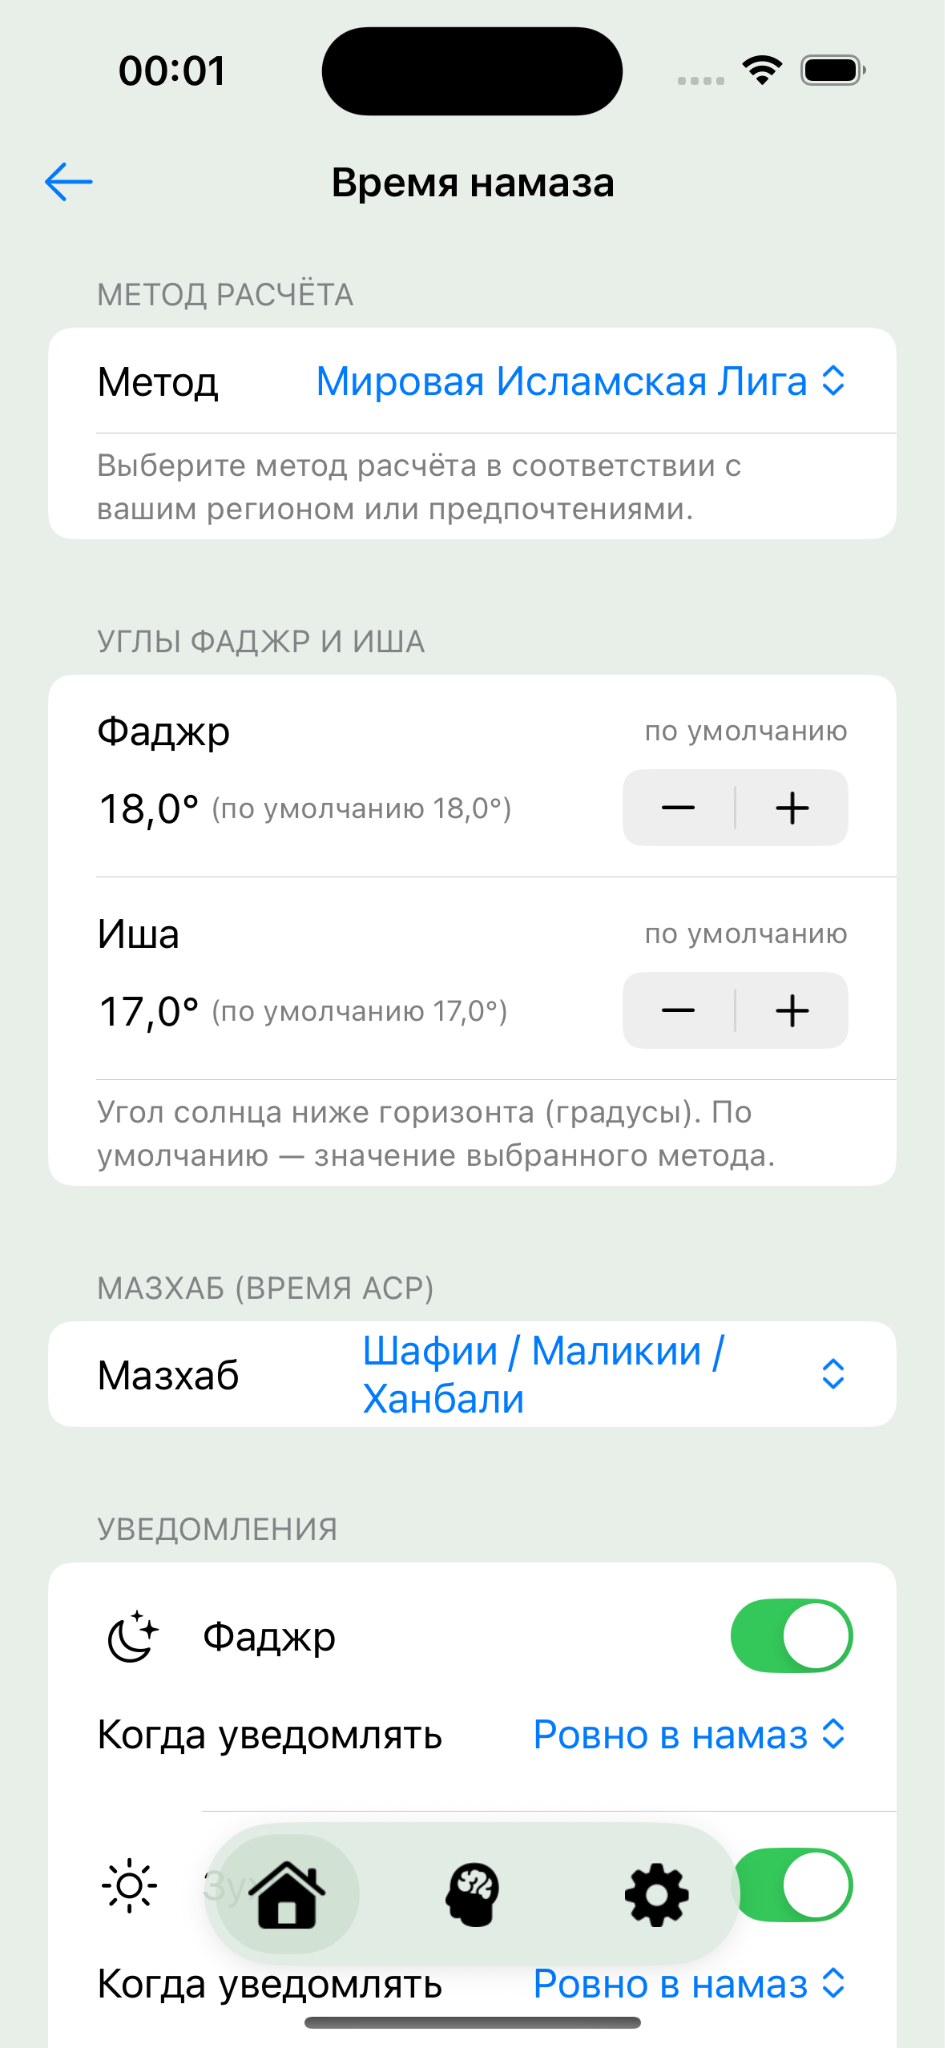
\includegraphics[width=0.85\linewidth, height=0.85\textheight, keepaspectratio]{my_folder/images/image55}
	\caption{Реализованный экран настройки уведомлений о времени молитвы}
	\label{fig:55}
\end{figure}


\begin{figure}[H]
	\centering
	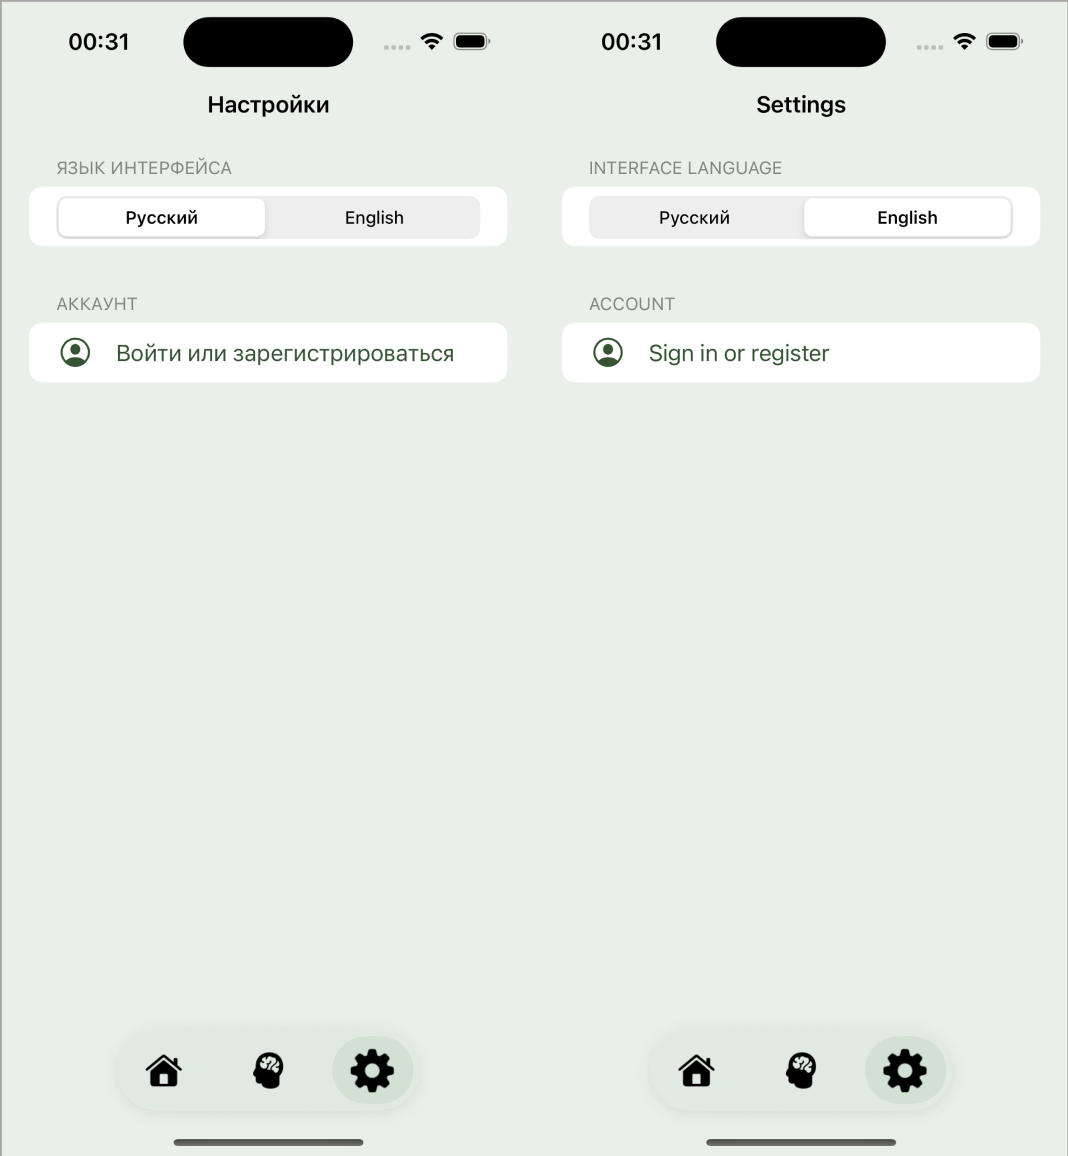
\includegraphics[width=0.85\linewidth]{my_folder/images/image56}
	\caption{Реализованный экран настройки выбора языка}
	\label{fig:56}
\end{figure}


\begin{figure}[H]
	\centering
	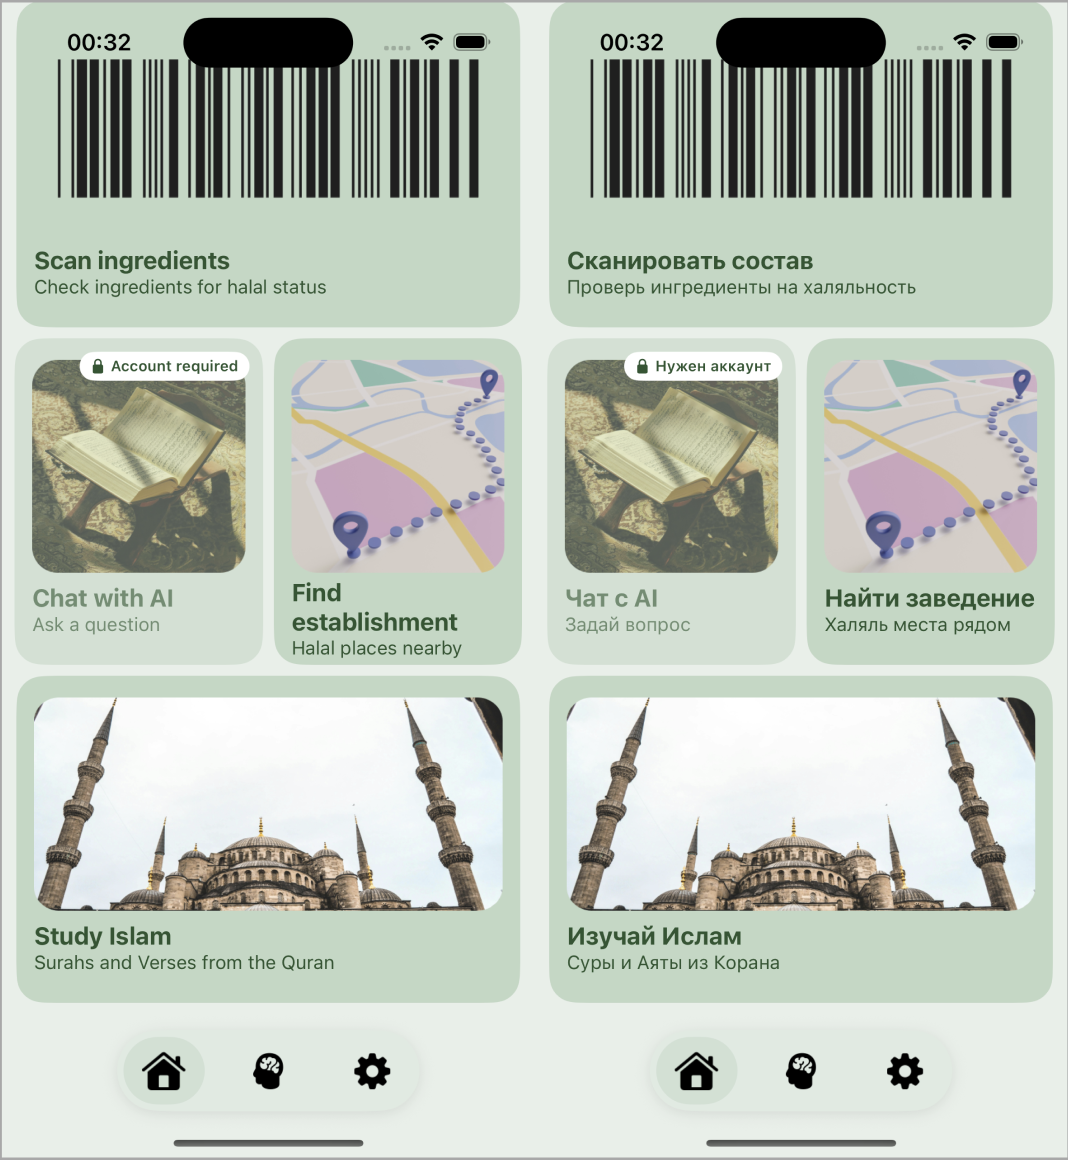
\includegraphics[width=0.85\linewidth]{my_folder/images/image57}
	\caption{Главный экран на русском и английском языке}
	\label{fig:57}
\end{figure}


\subsection{Проверка производительности системы}


Проверка производительности проводилась с целью подтверждения соответствия времени отклика компонентов установленным требованиям. Тестирование охватывало три основных компонента системы: backend-приложение, LLM-сервис и мобильное iOS-приложение.


В рамках работы использовался подход SLA-тестирования (Service Level Agreement), при котором измеряется время выполнения конкретной операции и сравнивается с заранее установленным пороговым значением. В отличие от полноценного нагрузочного тестирования, данный подход позволяет проверить производительность приложения без необходимости разворачивания продуктивной инфраструктуры и внешних сервисов.


Для тестирования были выбраны следующие SLA-пороги:

\begin{enumerate}
	\item операции аутентификации (/api/auth/*) - не более 500 мс.
	\item чат-запросы (/api/chat, /llm/chat) - не более 2 000 мс.
	\item справочные эндпоинты (/api/models, /llm/info) - не более 200 мс.
	\item health-check эндпоинты - не более 100 мс.
	\item синхронные клиентские операции iOS - не более 50 мс.
\end{enumerate}

На стороне backend были реализованы тесты производительности с использованием JUnit 5 и MockMvc. Проверялось время выполнения операций регистрации, входа пользователя, обновления JWT-токена, получения списка моделей и отправки чат-запросов. Дополнительно были реализованы тесты конкурентной нагрузки, в рамках которых несколько параллельных запросов должны были завершаться в пределах общего временного лимита. Это позволило проверить отсутствие существенной деградации производительности при одновременном выполнении нескольких операций (рисунок~\ref{fig:58}).


\begin{figure}[H]
	\centering
	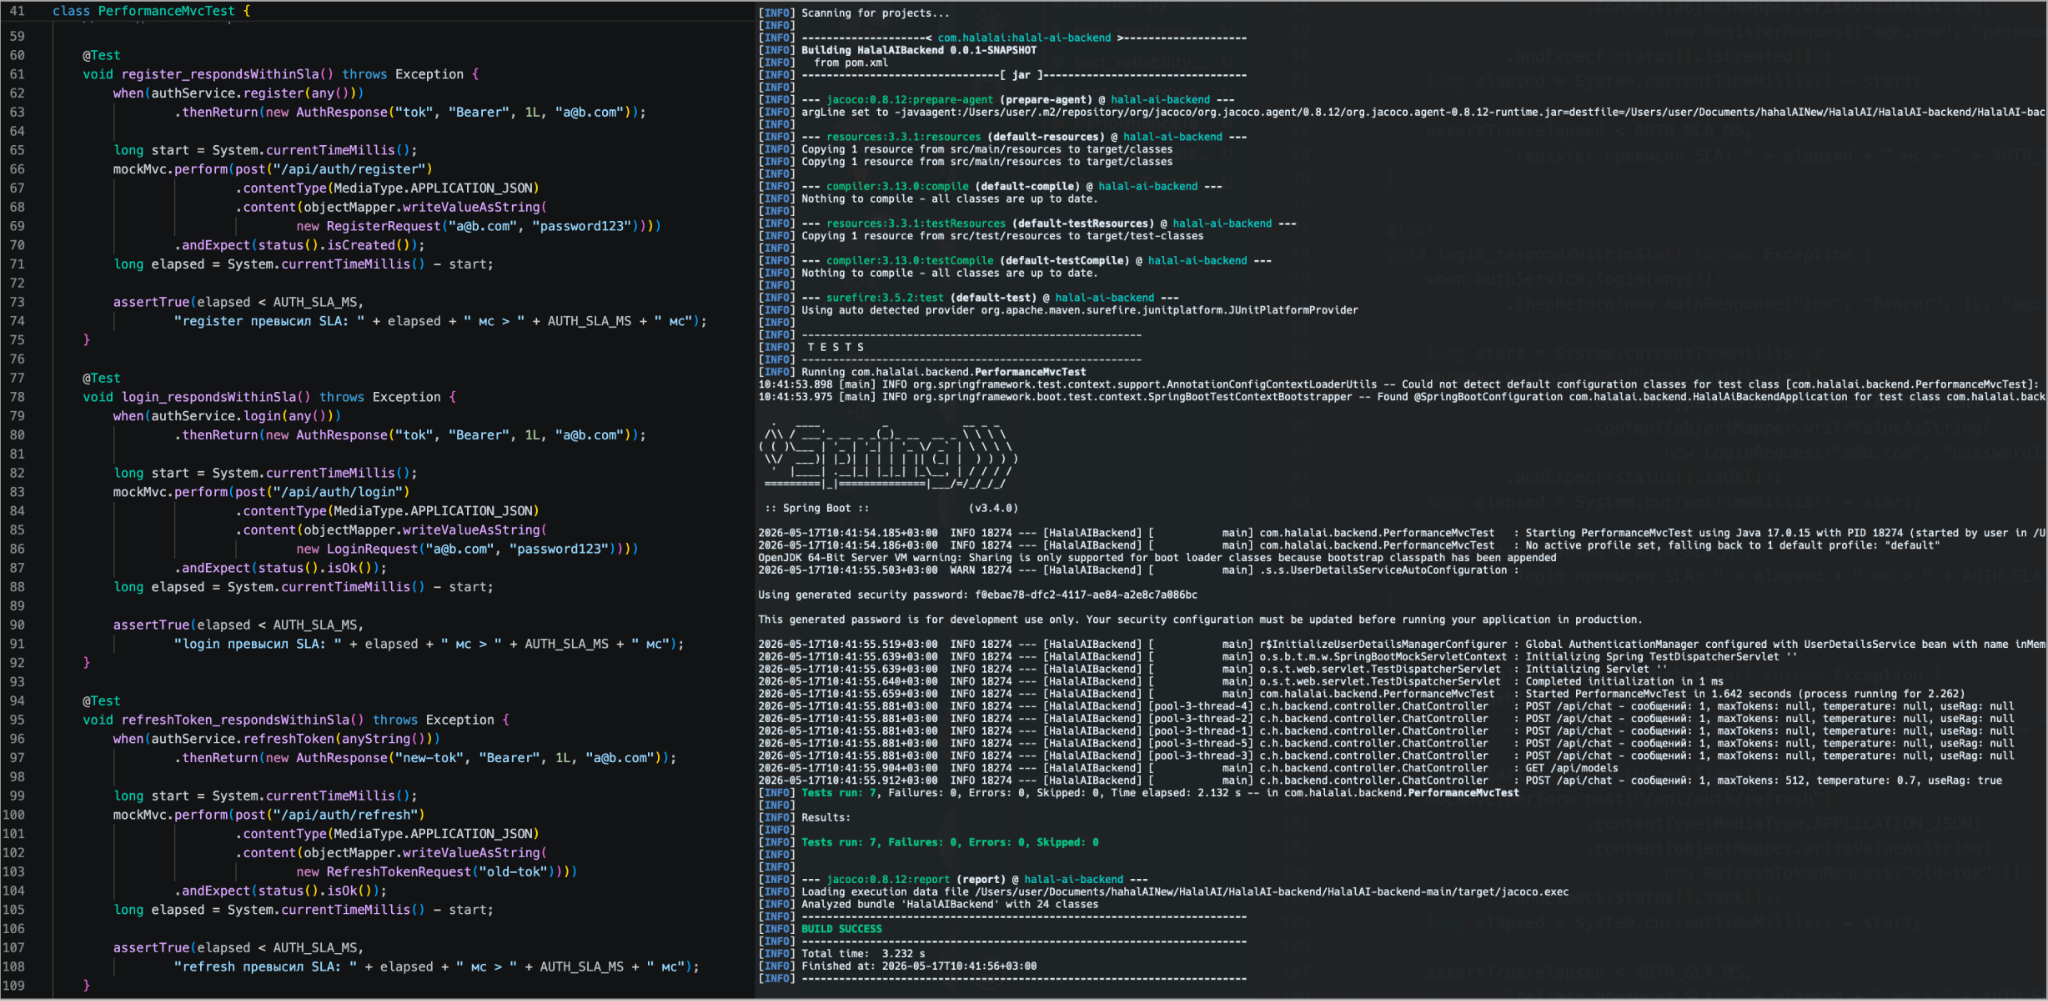
\includegraphics[width=0.85\linewidth]{my_folder/images/image58}
	\caption{Тестирование производительности backend}
	\label{fig:58}
\end{figure}


Для LLM-сервиса на FastAPI использовались pytest и FastAPI TestClient. В тестах измерялось время ответа эндпоинтов /llm/health, /llm/info и /llm/chat. Поскольку реальные обращения к внешним LLM-провайдерам обладают высокой сетевой задержкой и зависят от внешней инфраструктуры, OpenRouter-клиент был заменён mock-объектом. Это позволило измерять производительность непосредственно HTTP-слоя и бизнес-логики приложения (рисунок~\ref{fig:59}).


\begin{figure}[H]
	\centering
	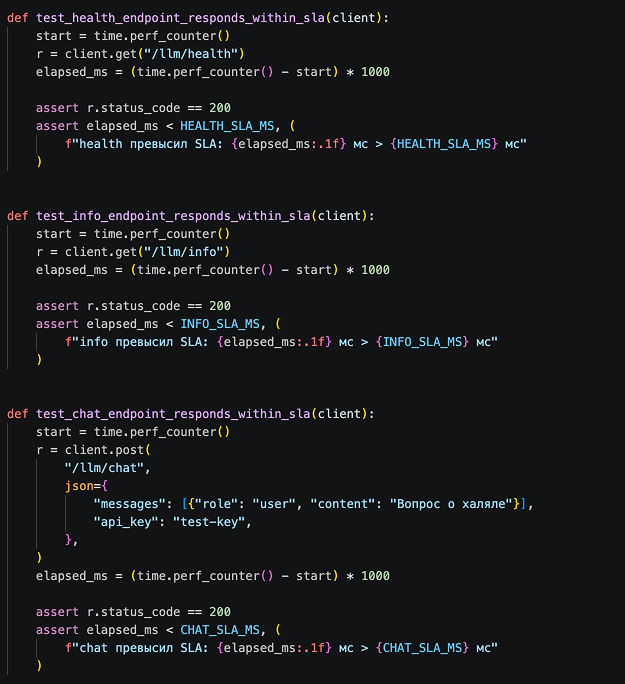
\includegraphics[width=0.85\linewidth]{my_folder/images/image59}
	\caption{Тесты производительности LLM-сервиса}
	\label{fig:59}
\end{figure}


В iOS производительность проверялась с использованием Swift Testing и ContinuousClock.measure. Тестировалось время выполнения операций авторизации, регистрации, обновления токена, загрузки списка моделей, а также скорость локальных синхронных операций, связанных с обновлением состояния интерфейса. Особое внимание уделялось тому, чтобы операции изменения состояния чата не блокировали основной UI-поток (рисунок~\ref{fig:60}).


\begin{figure}[H]
	\centering
	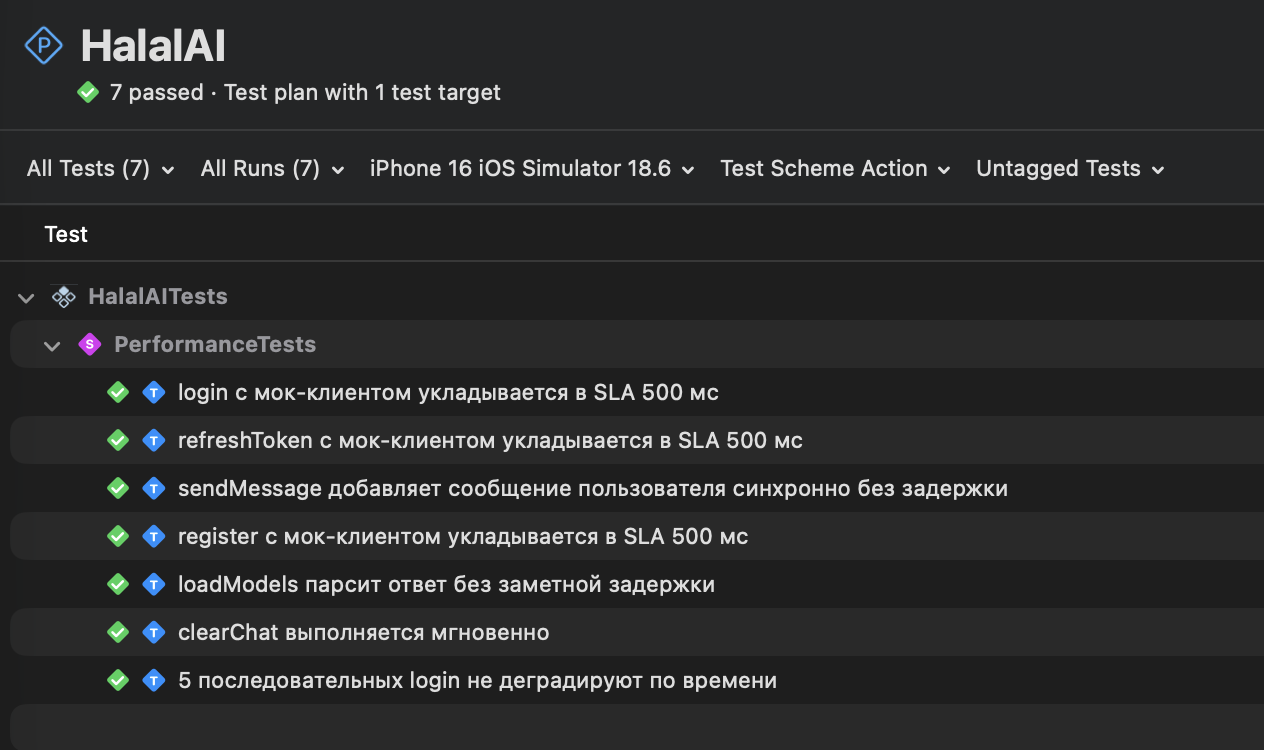
\includegraphics[width=0.85\linewidth]{my_folder/images/image60}
	\caption{Пройденные тесты производительности iOS}
	\label{fig:60}
\end{figure}


Всего для проверки производительности было реализовано 20 автоматизированных тестов:

\begin{enumerate}
	\item 7 тестов для backend.
	\item 6 тестов для LLM-сервиса.
	\item 7 тестов для iOS-приложения.
\end{enumerate}

Результаты тестирования показали, что все реализованные операции укладываются в установленные SLA-пороговые значения. Это подтверждает, что архитектура системы и выбранные технологии обеспечивают достаточную производительность для использования в мобильном приложении.


\subsection{Проверка надежности системы}


Проверка надежности проводилась с целью оценки устойчивости приложения к ошибкам, сбоям внешних сервисов и некорректным входным данным. Основная задача тестирования заключалась в подтверждении того, что система сохраняет работоспособность и корректно обрабатывает исключительные ситуации без аварийного завершения работы.


В ходе тестирования проверялись следующие свойства надежности:

\begin{enumerate}
	\item корректная деградация при отказе внешних сервисов.
	\item независимость компонентов системы.
	\item восстановление после временных сбоев.
	\item устойчивость к повторным ошибочным запросам.
	\item отсутствие критических сбоев приложения при некорректных данных.
\end{enumerate}

На стороне backend были реализованы тесты с использованием JUnit 5 и MockMvc. Проверялись сценарии недоступности LLM-сервиса, возврата ошибок со стороны внешних зависимостей, повторных неудачных запросов и восстановления после временного отказа. Например, при выбросе исключения со стороны LLM-сервиса backend должен был возвращать структурированный JSON-ответ с кодом ошибки, а не необработанный 500 Internal Server Error. Также проверялось, что отказ чат-сервиса не влияет на доступность эндпоинтов аутентификации (рисунок~\ref{fig:61}).


\begin{figure}[H]
	\centering
	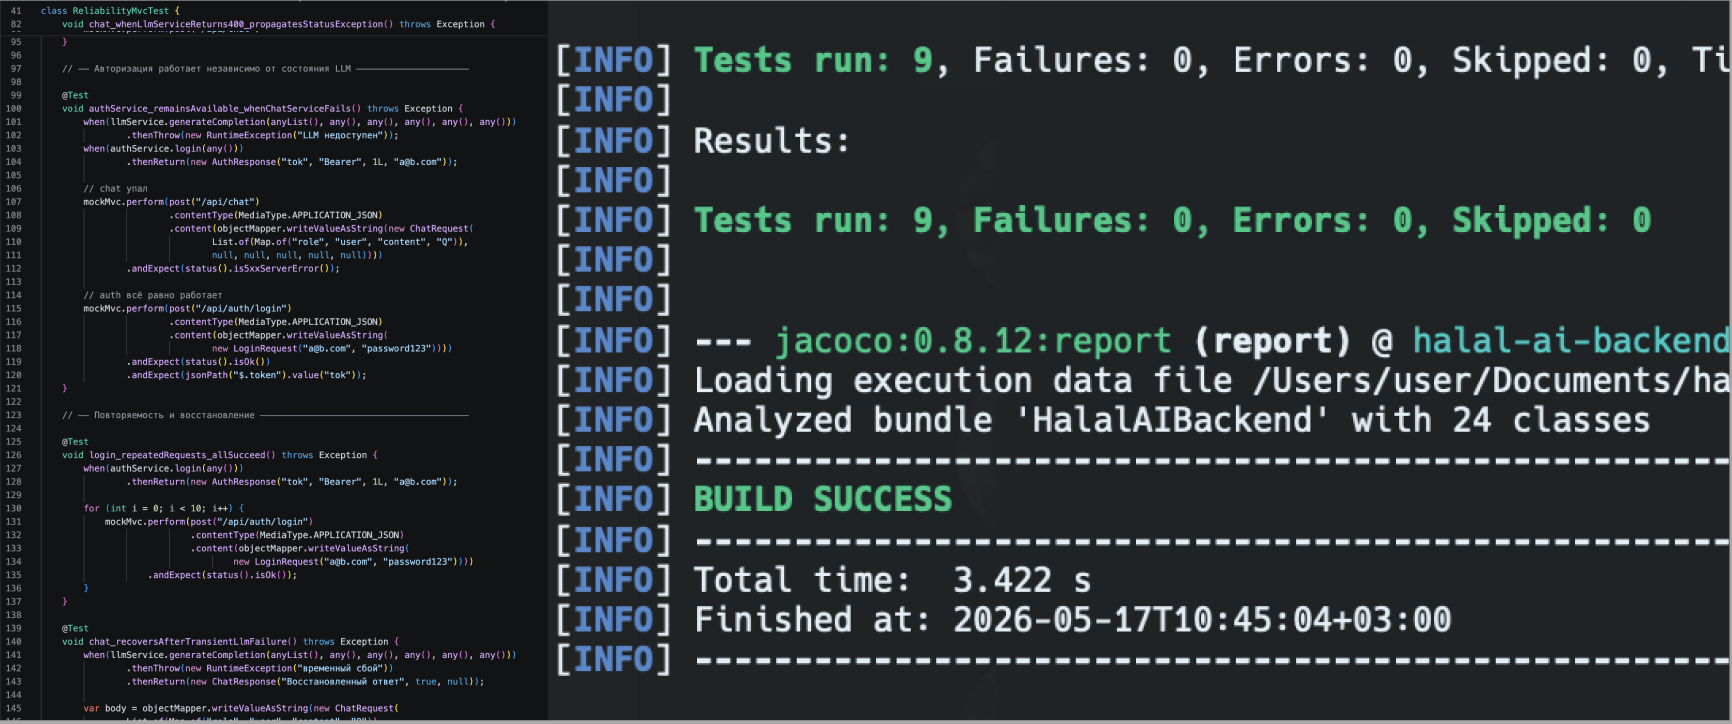
\includegraphics[width=0.85\linewidth]{my_folder/images/image61}
	\caption{Тесты надежности backend}
	\label{fig:61}
\end{figure}


Для LLM-сервиса тестирование проводилось с использованием pytest и FastAPI TestClient. Проверялись сценарии неинициализированного сервиса, ошибок со стороны OpenRouter, пустых сообщений, последовательных запросов и восстановления после временных сбоев. Важным требованием являлось отсутствие необработанных исключений и корректное возвращение HTTP-статусов (рисунки~\ref{fig:62},~\ref{fig:63}).


\begin{figure}[H]
	\centering
	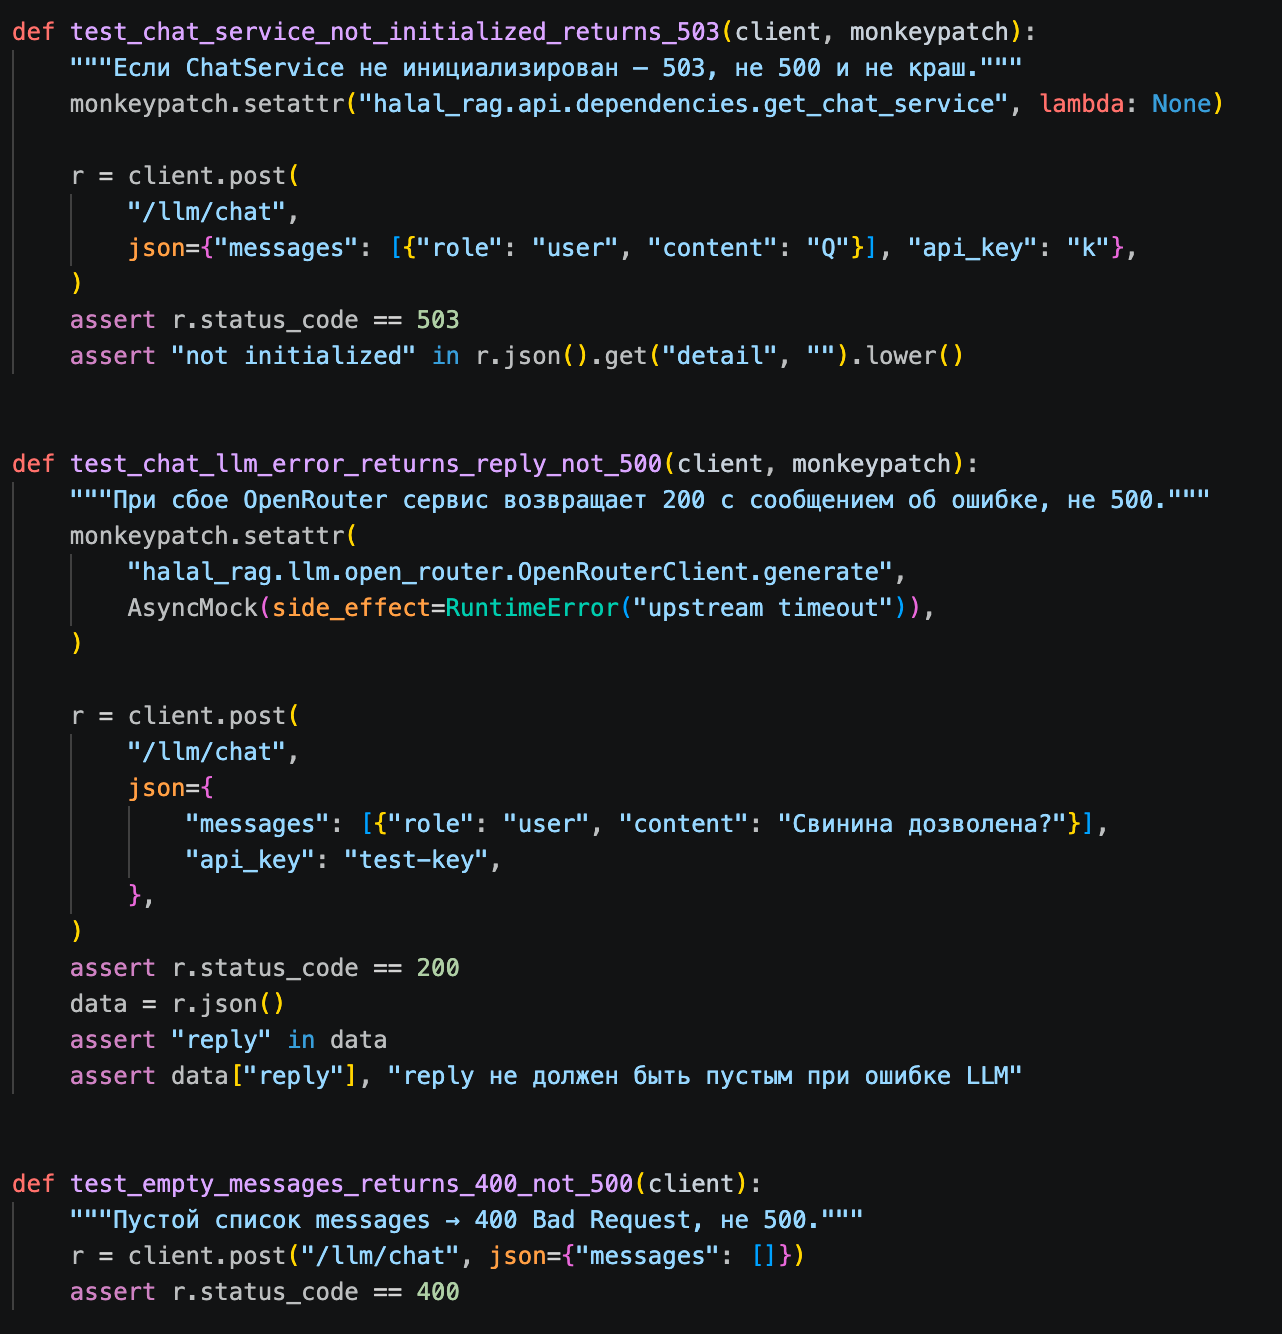
\includegraphics[width=0.85\linewidth]{my_folder/images/image62}
	\caption{Тесты надежности LLM-сервиса}
	\label{fig:62}
\end{figure}


\begin{figure}[H]
	\centering
	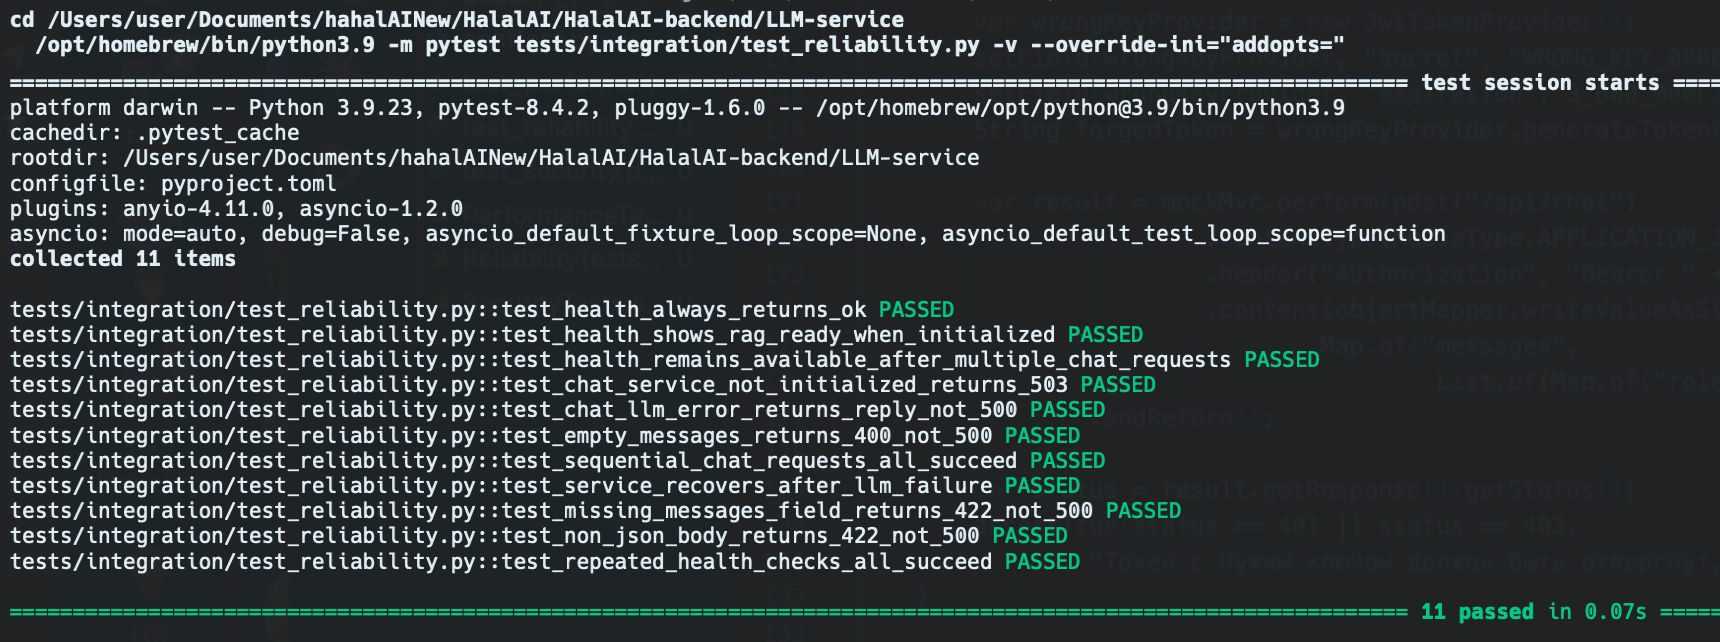
\includegraphics[width=0.85\linewidth]{my_folder/images/image63}
	\caption{Пройденные тесты надежности LLM-сервиса}
	\label{fig:63}
\end{figure}


В мобильном приложении iOS проверялась устойчивость клиентской логики к сетевым ошибкам и сбоям API. Тесты подтвердили, что:

\begin{enumerate}
	\item приложение не завершается аварийно при отсутствии сети.
	\item состояние isLoading всегда корректно сбрасывается после ошибки.
	\item повторные ошибки не приводят к деградации состояния ViewModel.
	\item после успешного запроса приложение корректно восстанавливается после предыдущего сбоя.
	\item очистка состояния чата и выход из аккаунта корректно восстанавливают исходное состояние приложения.
\end{enumerate}

Особое внимание уделялось сценариям, связанным с пользовательским интерфейсом. Для мобильного приложения критично, чтобы даже при ошибках серверной части интерфейс не переходил в "зависшее" состояние (рисунок~\ref{fig:64}).


\begin{figure}[H]
	\centering
	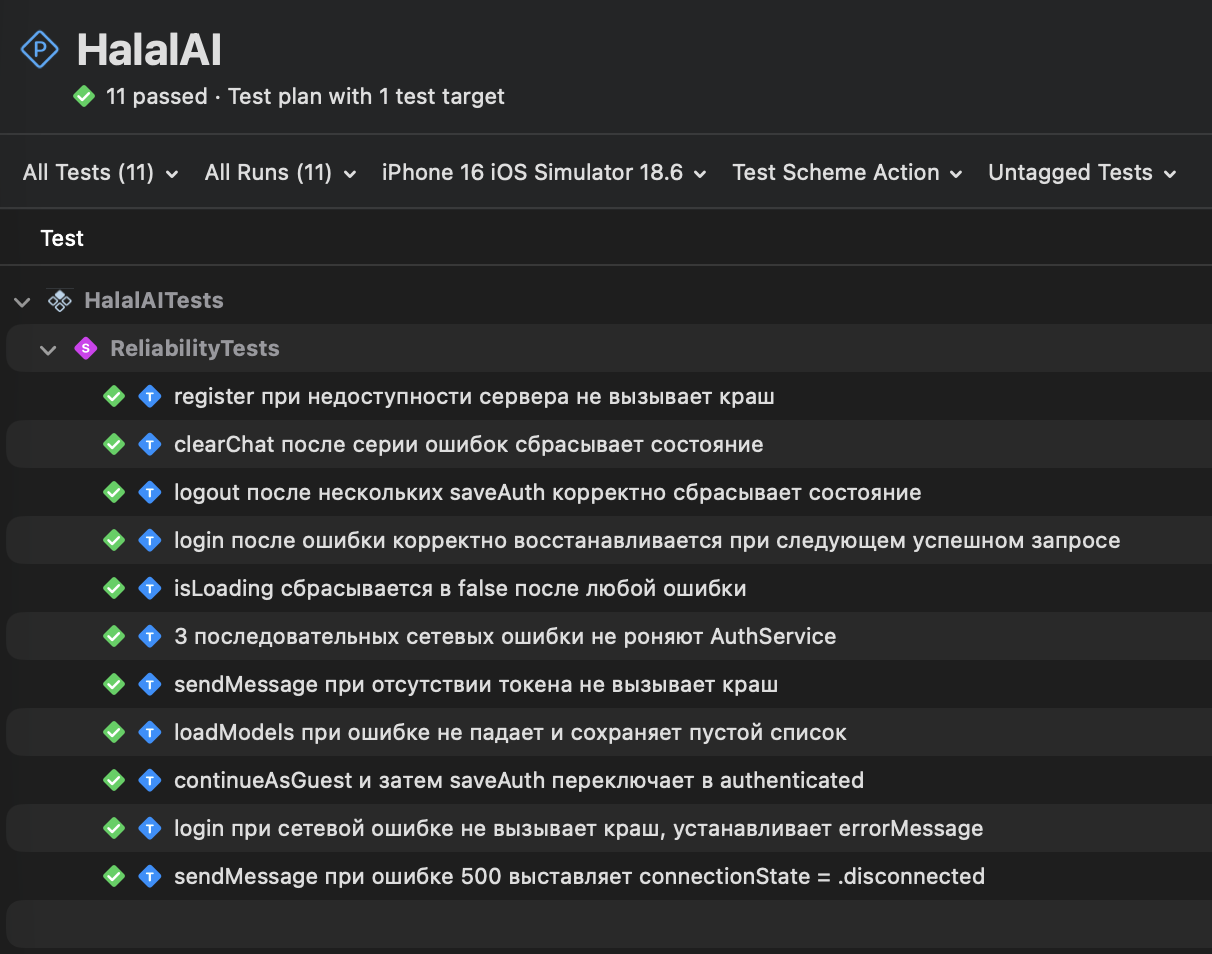
\includegraphics[width=0.85\linewidth]{my_folder/images/image64}
	\caption{Пройденные тесты надежности iOS}
	\label{fig:64}
\end{figure}


Всего для проверки надежности было реализовано 29 автоматизированных тестов:

\begin{enumerate}
	\item 9 тестов для backend.
	\item 10 тестов для LLM-сервиса.
	\item 10 тестов для iOS-приложения.
\end{enumerate}

Результаты тестирования показали, что система корректно обрабатывает сбои, не завершается аварийно и способна восстанавливаться после временных ошибок. Это подтверждает устойчивость реализованной архитектуры и корректную обработку исключительных ситуаций на всех уровнях системы.


\subsection{Проверка безопасности}


Проверка безопасности системы проводилась с целью подтверждения корректной реализации механизмов аутентификации, контроля доступа и обработки потенциально опасных входных данных.


Тестирование безопасности охватывало три направления:

\begin{enumerate}
	\item контроль доступа к защищенным ресурсам.
	\item корректную работу механизма JWT-аутентификации.
	\item устойчивость системы к некорректным и потенциально вредоносным данным.
\end{enumerate}

Для backend-приложения были реализованы тесты на основе JUnit 5, MockMvc и Spring Security. В отличие от большинства тестов проекта, данные тесты выполнялись с использованием реальной цепочки фильтров Spring Security. Это позволило проверить фактическую работу механизмов авторизации и JWT-фильтрации.


В ходе тестирования проверялись следующие сценарии:

\begin{enumerate}
	\item доступ к защищённым эндпоинтам без JWT-токена.
	\item использование некорректного JWT.
	\item использование просроченного токена.
	\item использование токена, подписанного неправильным ключом.
	\item попытки передачи SQL-инъекций в заголовке Authorization.
	\item доступ к публичным эндпоинтам без авторизации.
	\item корректная работа CORS-заголовков.
\end{enumerate}

Результаты тестирования безопасности backend приведены на рисунках~\ref{fig:65} и~\ref{fig:66}.

\begin{figure}[H]
	\centering
	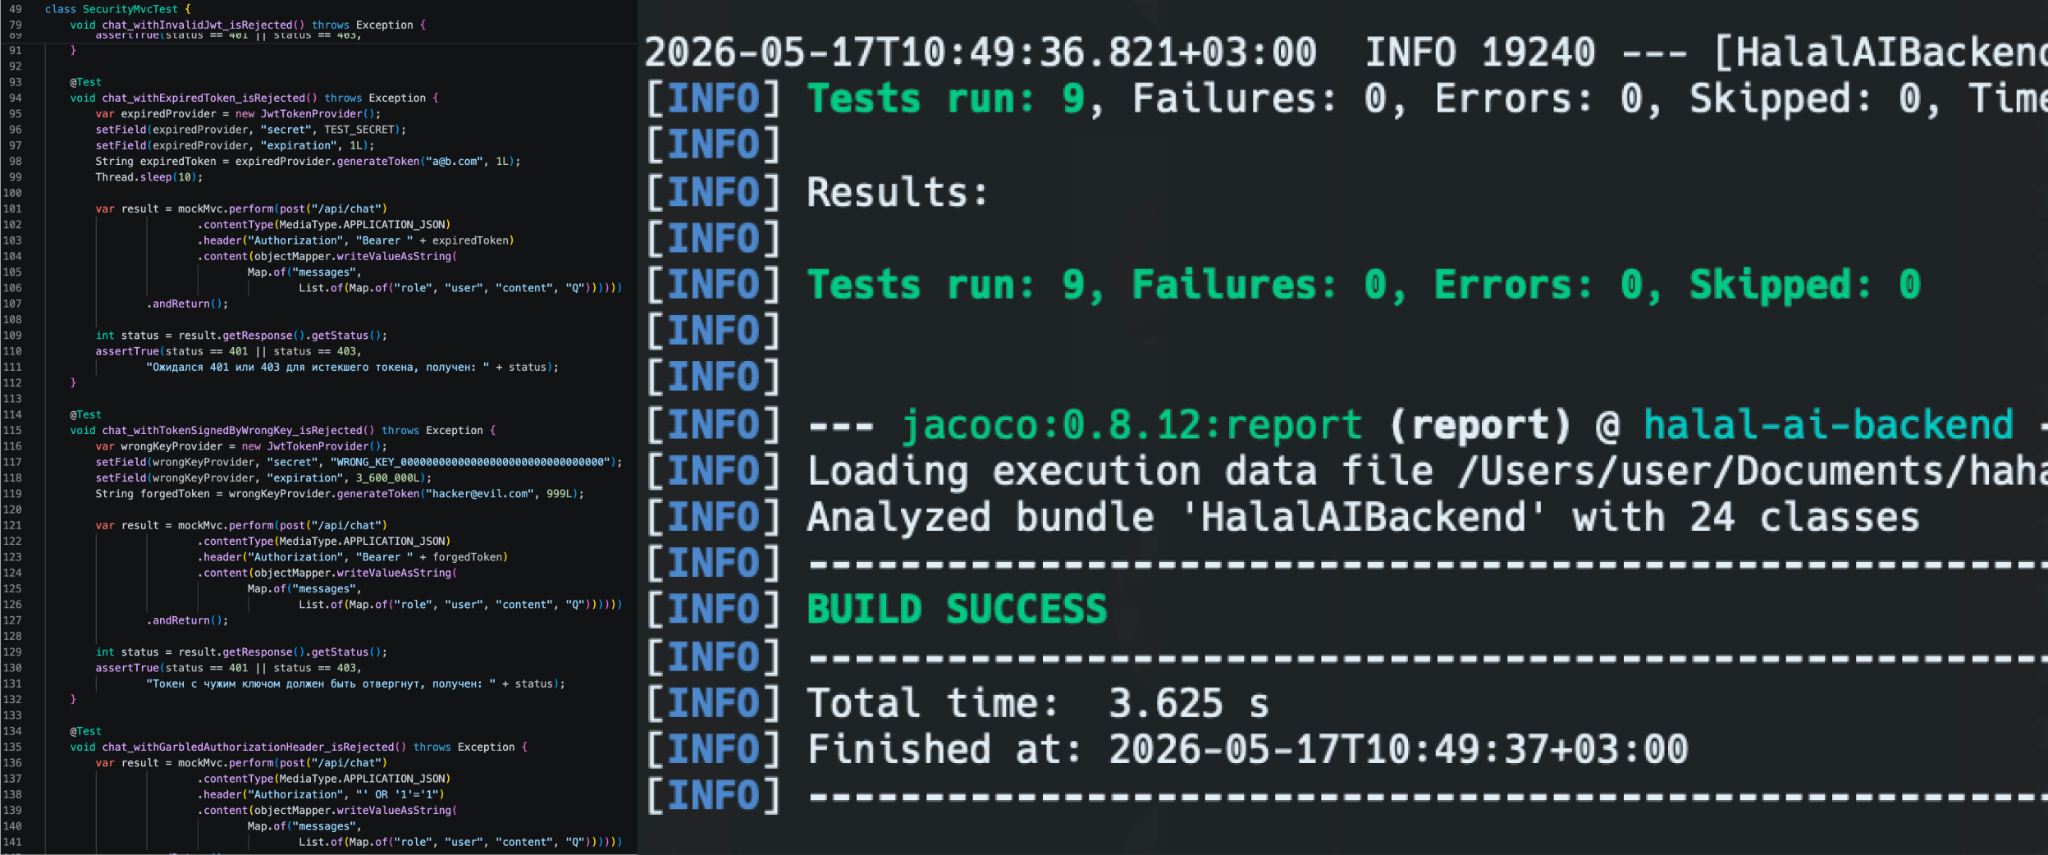
\includegraphics[width=0.85\linewidth]{my_folder/images/image65}
	\caption{Пройденные тесты безопасности backend}
	\label{fig:65}
\end{figure}


\begin{figure}[H]
	\centering
	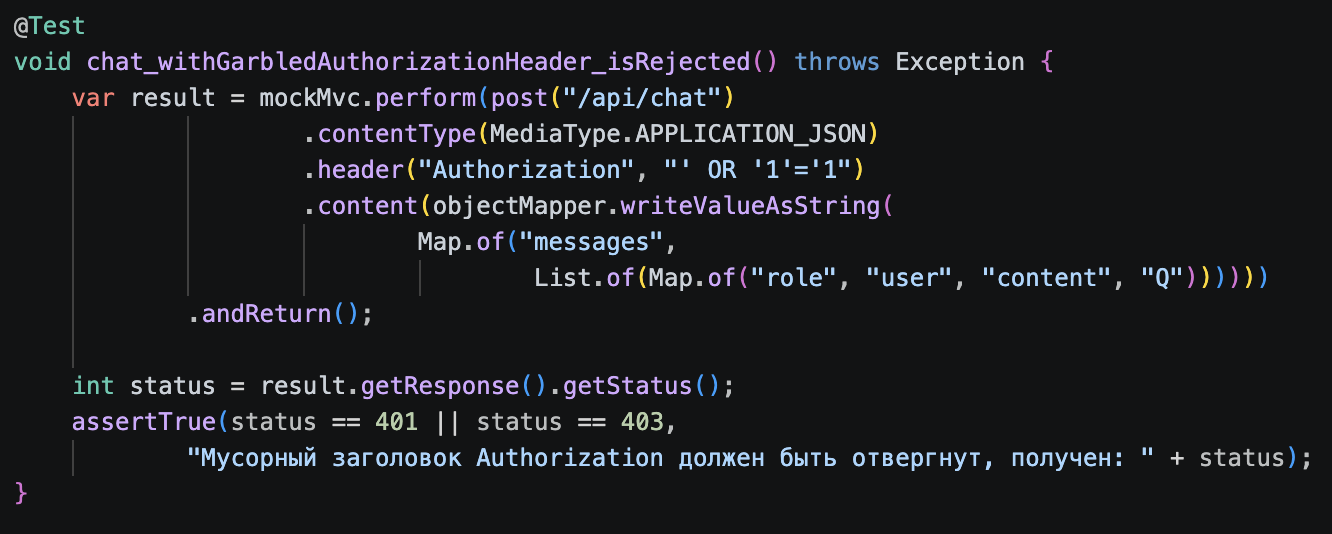
\includegraphics[width=0.85\linewidth]{my_folder/images/image66}
	\caption{Тесты на попытку передачи SQL-инъекций в заголовке Authorization}
	\label{fig:66}
\end{figure}


Отдельно проверялось, что только корректно подписанный JWT предоставляет доступ к защищенным ресурсам системы.


Для LLM-сервиса были реализованы тесты безопасности с использованием pytest. Проверялась устойчивость сервиса к различным типам вредоносных входных данных:

\begin{enumerate}
	\item SQL-инъекциям.
	\item XSS-строкам.
	\item shell-инъекциям.
	\item чрезмерно большим payload.
	\item некорректным Unicode-символам.
	\item null-значениям.
	\item отсутствующим обязательным полям.
\end{enumerate}

Главным критерием являлось отсутствие внутренних ошибок сервера (500 Internal Server Error) даже при передаче потенциально опасных данных. Сервис должен был либо успешно обработать запрос, либо вернуть ошибку валидации (400, 422, 413) (рисунки~\ref{fig:67},~\ref{fig:68}).


\begin{figure}[H]
	\centering
	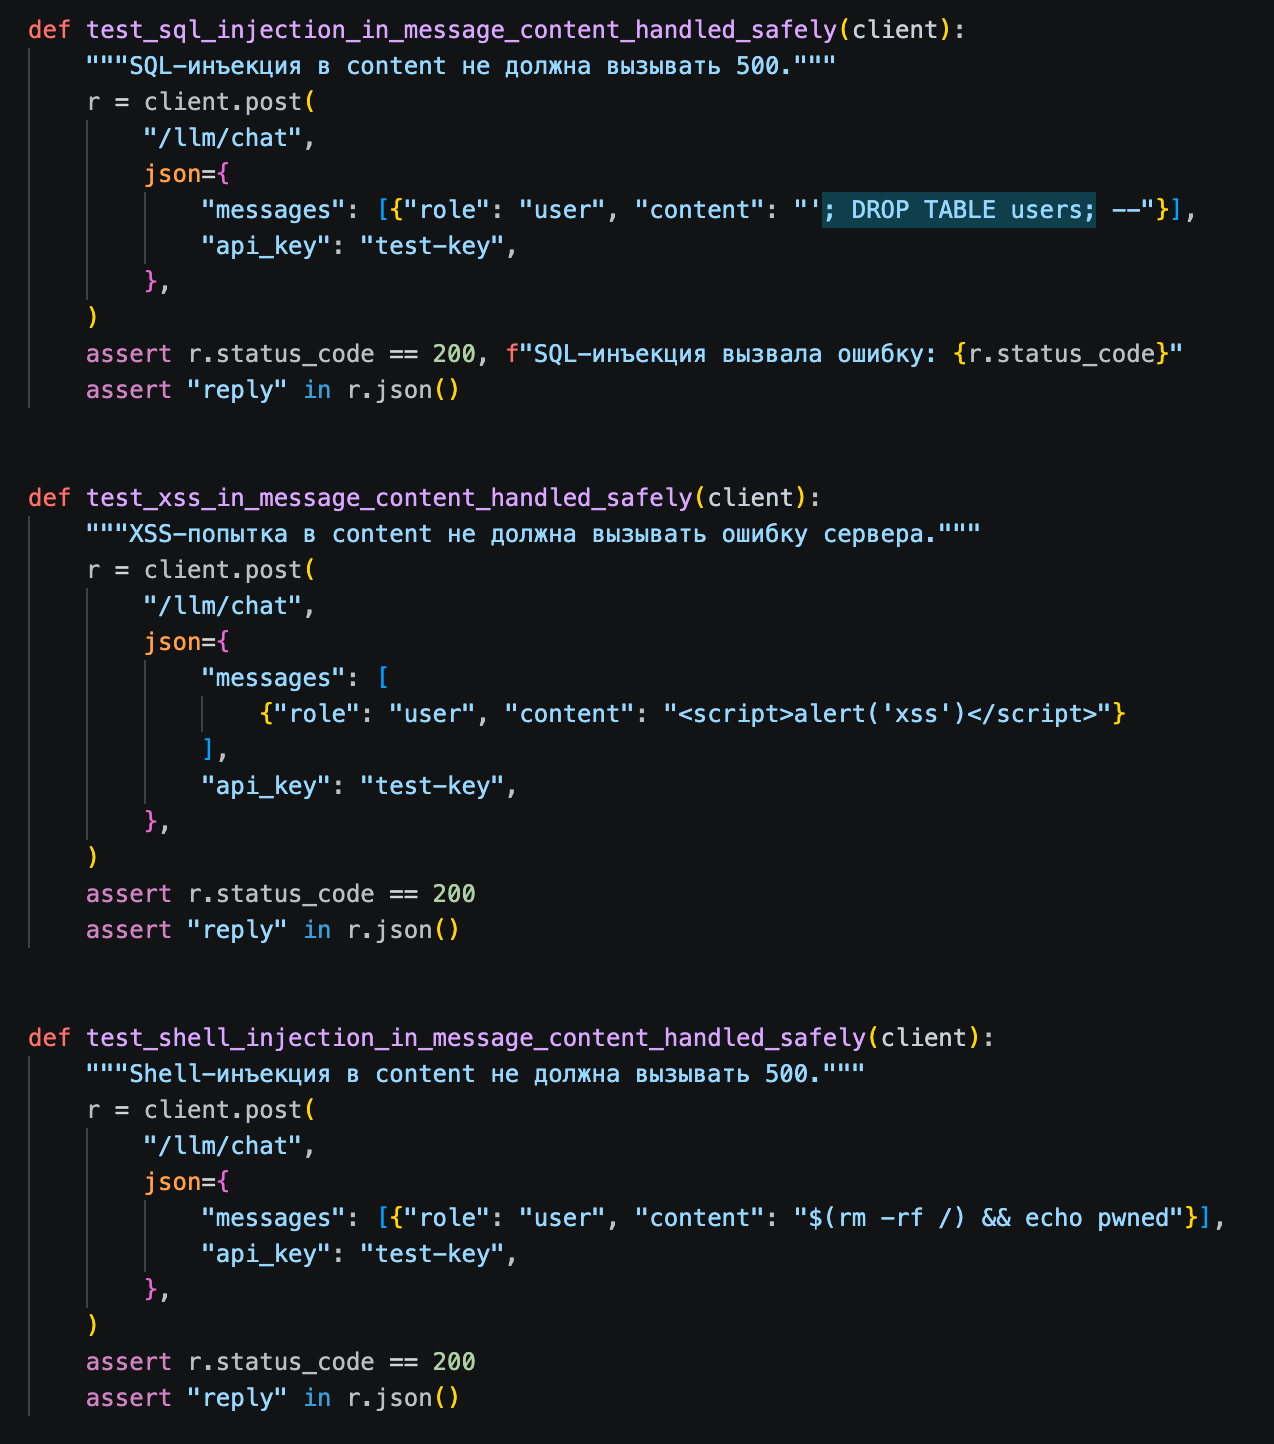
\includegraphics[width=0.85\linewidth]{my_folder/images/image67}
	\caption{Тесты безопасности LLM-сервиса}
	\label{fig:67}
\end{figure}


\begin{figure}[H]
	\centering
	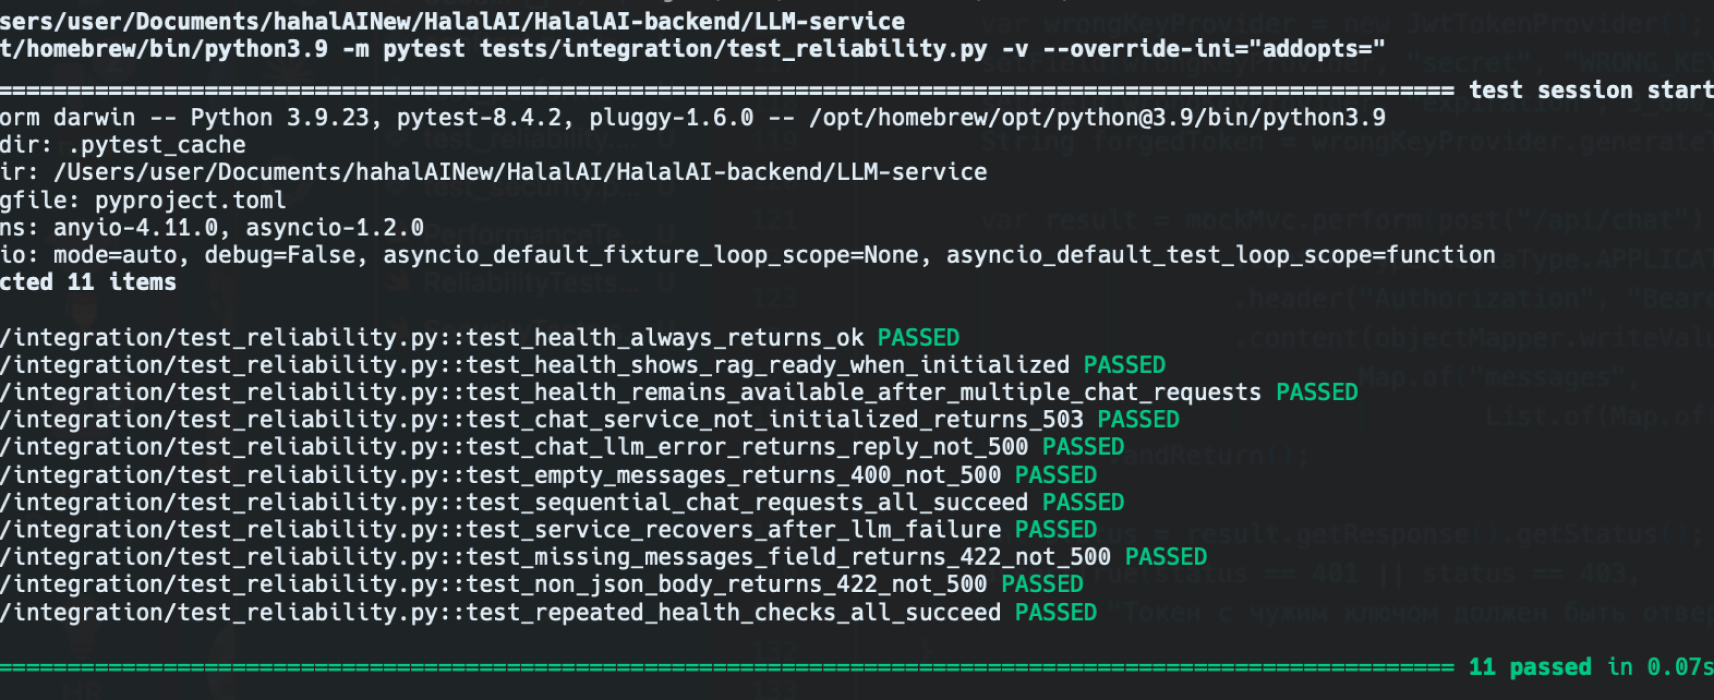
\includegraphics[width=0.85\linewidth]{my_folder/images/image68}
	\caption{Пройденные тесты безопасности LLM-сервиса}
	\label{fig:68}
\end{figure}


В iOS-приложении проверялись механизмы хранения и удаления токенов аутентификации, а также защита клиентской логики от некорректных пользовательских данных. Проверялось:

\begin{enumerate}
	\item отсутствие токена до авторизации;
	\item корректное сохранение JWT после входа;
	\item полное удаление токена и пользовательских данных после logout;
	\item невозможность отправки API-запросов без токена;
	\item защита от некорректных email-адресов и слишком длинных строк;
	\item устойчивость к SQL-инъекциям и XSS-строкам в полях ввода;
	\item ограничение диапазонов параметров генерации (maxTokens, temperature).
\end{enumerate}

Результаты тестирования безопасности iOS показаны на рисунке~\ref{fig:69}.

\begin{figure}[H]
	\centering
	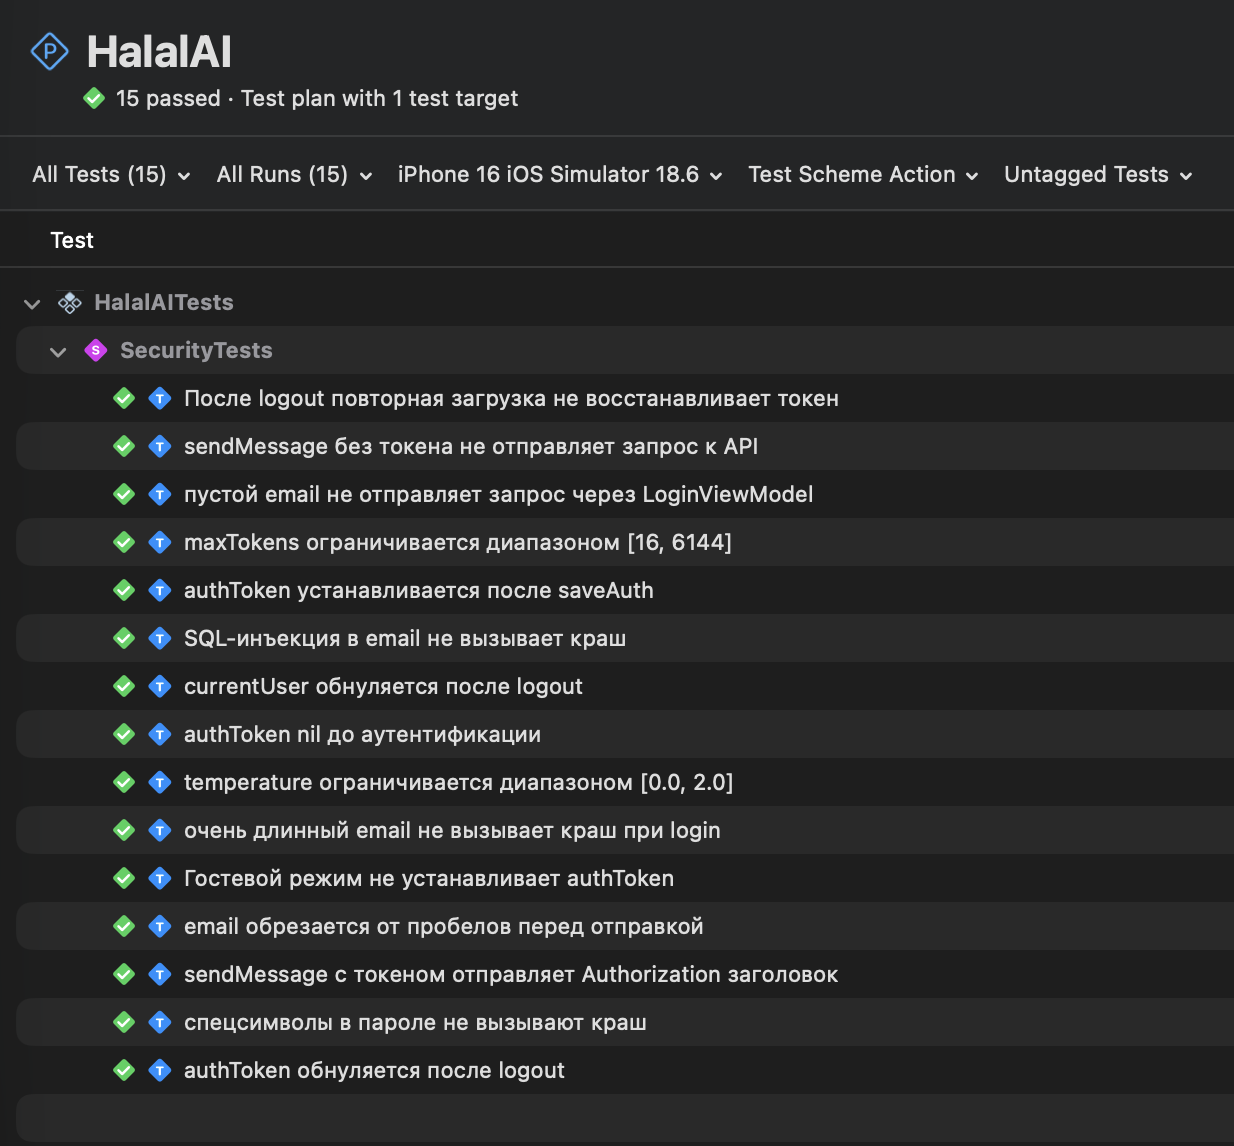
\includegraphics[width=0.85\linewidth]{my_folder/images/image69}
	\caption{Пройденные тесты безопасности iOS}
	\label{fig:69}
\end{figure}


Всего для проверки безопасности было реализовано 34 автоматизированных теста:

\begin{enumerate}
	\item 9 тестов для backend.
	\item 11 тестов для LLM-сервиса.
	\item 14 тестов для iOS-приложения.
\end{enumerate}

Результаты тестирования подтвердили корректную реализацию механизмов аутентификации и контроля доступа, а также устойчивость системы к некорректным и потенциально опасным входным данным. Дополнительно было установлено, что backend-приложение корректно использует цепочку фильтров Spring Security и действительно блокирует несанкционированный доступ к защищенным ресурсам.
